\documentclass[12pt,]{article}
\usepackage[T1]{fontenc}
\usepackage{lmodern}
\usepackage{amssymb,amsmath}
\usepackage{ifxetex,ifluatex}
\usepackage{fixltx2e} % provides \textsubscript
% Set line spacing
% use upquote if available, for straight quotes in verbatim environments
\IfFileExists{upquote.sty}{\usepackage{upquote}}{}
\ifnum 0\ifxetex 1\fi\ifluatex 1\fi=0 % if pdftex
  \usepackage[utf8]{inputenc}
\else % if luatex or xelatex
  \ifxetex
    \usepackage{mathspec}
    \usepackage{xltxtra,xunicode}
  \else
    \usepackage{fontspec}
  \fi
  \defaultfontfeatures{Mapping=tex-text,Scale=MatchLowercase}
  \newcommand{\euro}{€}
\fi
% use microtype if available
\IfFileExists{microtype.sty}{\usepackage{microtype}}{}
\usepackage[margin=1in]{geometry}
\usepackage{color}
\usepackage{fancyvrb}
\newcommand{\VerbBar}{|}
\newcommand{\VERB}{\Verb[commandchars=\\\{\}]}
\DefineVerbatimEnvironment{Highlighting}{Verbatim}{commandchars=\\\{\}}
% Add ',fontsize=\small' for more characters per line
\usepackage{framed}
\definecolor{shadecolor}{RGB}{248,248,248}
\newenvironment{Shaded}{\begin{snugshade}}{\end{snugshade}}
\newcommand{\KeywordTok}[1]{\textcolor[rgb]{0.13,0.29,0.53}{\textbf{{#1}}}}
\newcommand{\DataTypeTok}[1]{\textcolor[rgb]{0.13,0.29,0.53}{{#1}}}
\newcommand{\DecValTok}[1]{\textcolor[rgb]{0.00,0.00,0.81}{{#1}}}
\newcommand{\BaseNTok}[1]{\textcolor[rgb]{0.00,0.00,0.81}{{#1}}}
\newcommand{\FloatTok}[1]{\textcolor[rgb]{0.00,0.00,0.81}{{#1}}}
\newcommand{\CharTok}[1]{\textcolor[rgb]{0.31,0.60,0.02}{{#1}}}
\newcommand{\StringTok}[1]{\textcolor[rgb]{0.31,0.60,0.02}{{#1}}}
\newcommand{\CommentTok}[1]{\textcolor[rgb]{0.56,0.35,0.01}{\textit{{#1}}}}
\newcommand{\OtherTok}[1]{\textcolor[rgb]{0.56,0.35,0.01}{{#1}}}
\newcommand{\AlertTok}[1]{\textcolor[rgb]{0.94,0.16,0.16}{{#1}}}
\newcommand{\FunctionTok}[1]{\textcolor[rgb]{0.00,0.00,0.00}{{#1}}}
\newcommand{\RegionMarkerTok}[1]{{#1}}
\newcommand{\ErrorTok}[1]{\textbf{{#1}}}
\newcommand{\NormalTok}[1]{{#1}}
\usepackage{longtable,booktabs}
\usepackage{graphicx}
% Redefine \includegraphics so that, unless explicit options are
% given, the image width will not exceed the width of the page.
% Images get their normal width if they fit onto the page, but
% are scaled down if they would overflow the margins.
\makeatletter
\def\ScaleIfNeeded{%
  \ifdim\Gin@nat@width>\linewidth
    \linewidth
  \else
    \Gin@nat@width
  \fi
}
\makeatother
\let\Oldincludegraphics\includegraphics
{%
 \catcode`\@=11\relax%
 \gdef\includegraphics{\@ifnextchar[{\Oldincludegraphics}{\Oldincludegraphics[width=\ScaleIfNeeded]}}%
}%
\ifxetex
  \usepackage[setpagesize=false, % page size defined by xetex
              unicode=false, % unicode breaks when used with xetex
              xetex]{hyperref}
\else
  \usepackage[unicode=true]{hyperref}
\fi
\hypersetup{breaklinks=true,
            bookmarks=true,
            pdfauthor={Lisa MALIPHOL},
            pdftitle={Diateam SCAD@COPS A Hybrid Network Intrusion Detection System},
            colorlinks=true,
            citecolor=blue,
            urlcolor=blue,
            linkcolor=magenta,
            pdfborder={0 0 0}}
\urlstyle{same}  % don't use monospace font for urls
\setlength{\parindent}{0pt}
\setlength{\parskip}{6pt plus 2pt minus 1pt}
\setlength{\emergencystretch}{3em}  % prevent overfull lines
\setcounter{secnumdepth}{5}

%%% Change title format to be more compact
\usepackage{titling}
\setlength{\droptitle}{-2em}
  \title{Diateam\\SCAD@COPS\\A Hybrid Network Intrusion Detection System}
  \pretitle{\vspace{\droptitle}\centering\huge}
  \posttitle{\par}
  \author{Lisa MALIPHOL}
  \preauthor{\centering\large\emph}
  \postauthor{\par}
  \date{}
  \predate{}\postdate{}




\begin{document}

\maketitle


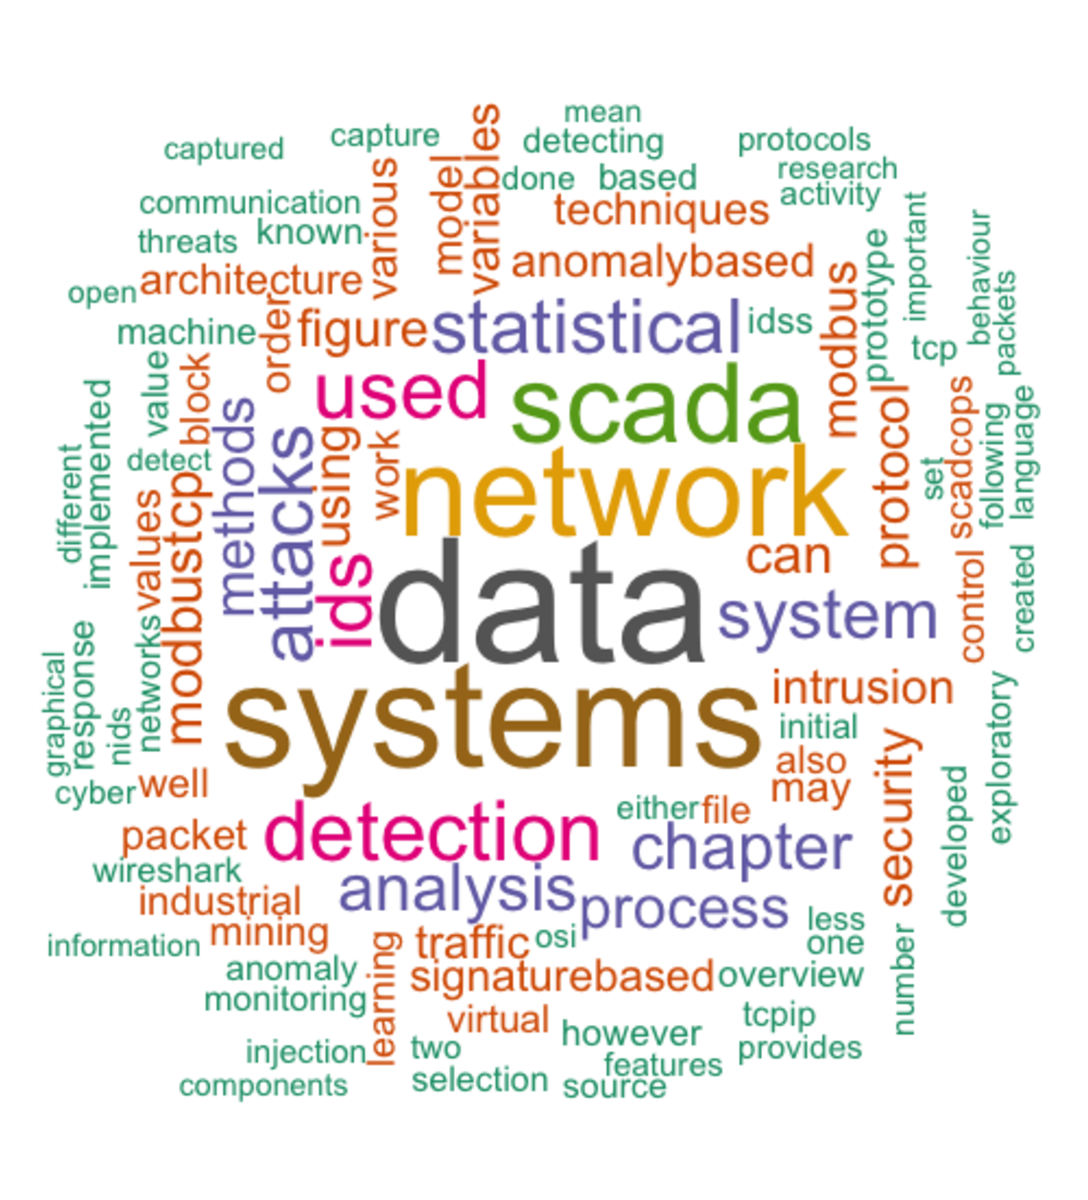
\includegraphics{thesis_files/figure-latex/unnamed-chunk-3-1.pdf}

\thispagestyle{empty}

\newpage
\thispagestyle{empty} \mbox{}

\clearpage
\pagenumbering{roman}

\begin{center}

\vspace{30mm}

{\Huge Diateam: SCAD@COPS}\\
\bigskip
{\Huge A Hybrid Network Intrusion Detection System}\\
\vspace{15mm}
{\Large by}\\

\vspace{18mm}
{\huge Lisa MALIPHOL}\\

\vspace{25mm}

\textit{A thesis submitted in partial satisfaction of the}\\
\medskip
\textit{requirements for the diploma of the}\\
\medskip
\textit{Masters of Science}\\
\medskip
\textit{in}\\
\medskip
\textit{Computer Science and Decision Systems}\\
\medskip
\textit{in the}\\
\medskip
\textit{Grande École}\\
\medskip
\textbf{\textit{\Large Télécom Bretagne}}\\

\vspace{10mm}

\textit{Academic Advisors:}\\
\medskip
\textit{Professor Yannis Haralambous}\\
\medskip
\textit{Professor Sandrine Vaton}\\

\vspace{15mm}

\textit{September 2015}\\
\medskip
\textit{Plouzane, FRANCE}\\

\end{center}

\thispagestyle{empty} \newpage
\mbox{} \thispagestyle{empty}

\newpage

\section*{Acknowledgements}\label{acknowledgements}
\addcontentsline{toc}{section}{Acknowledgements}

\newpage
\mbox{} \thispagestyle{empty}

\clearpage

\section*{Abstract}\label{abstract}
\addcontentsline{toc}{section}{Abstract}

\newpage
\mbox{} \thispagestyle{empty}

\clearpage

\section*{Résumé}\label{resume}
\addcontentsline{toc}{section}{Résumé}

\newpage
\mbox{} \thispagestyle{empty}

\clearpage

\tableofcontents

\cleardoublepage

\listoffigures

\newpage
\mbox{} \thispagestyle{empty}

\clearpage

\section*{Acronyms}\label{acronyms}
\addcontentsline{toc}{section}{Acronyms}

\begin{itemize}
\itemsep1pt\parskip0pt\parsep0pt
\item
  ANIDS - Anomoly-based Network Intrusion Detection System
\item
  HNS - Hybrid Network Simulation
\item
  HMI - Human-Machine Interface - a software and hardware designed for a
  human operator to monitor the state of a process under control, modify
  control settings and manually override automatic control operations
\item
  ICS - Industrial Control System
\item
  IDS - Intrusion Detection System
\item
  IPS - Intrusion Prevention System
\item
  MTU - Master Terminal Unit
\item
  PLC - Programmable Logic Controller - a small industrial computer
  designed to perform logic functions executed by electrical hardware
\item
  MTU - Master Terminal Unit
\item
  NIDS - Network Intrusion Detection System
\item
  RTU - Remote Terminal Unit - a field device that is a data acquisition
  and control unit designed to support SCADA remote stations
\item
  SCADA - Supervisory Control and Data Acquisition
\end{itemize}

\thispagestyle{empty} \newpage
\mbox{} \thispagestyle{empty}

\clearpage
\setcounter{page}{15} \pagenumbering{arabic}

\section{Introduction}\label{introduction}

Supervisory control and data acquisition systems (SCADA) are one type of
industrial control system (ICS) put in place for monitoring and
controlling industrial processes, such as those in the energy or
manufacturing sectors. Originally, these systems were isolated and used
proprietary protocols, whose security relied predominantly on obscurity.
As SCADA systems have moved towards open standards and have become more
interconnected to traditional information technology systems, these
critical systems have also become increasingly exposed and targeted to
cyber attacks.{[}Zhu2010{]}{[}Zhu2011{]}{[}1, 2{]}

To secure SCADA systems, intrusion detection systems (IDS) are put into
place with the purpose of observing, analyzing and detecting any
malicious activity, which are then alerted to, and reviewed by, security
analysts. Most IDSs found in the market-place are commonly network,
signature-based IDSs. Anomaly-based detection systems are relatively
immature, however, they provide a greater possibility of detecting
unknown attacks. Signature-based systems can only detect known and
identified signatures of attacks.

The trade-off between the two types of systems, signature-based and
anomaly-based, are predominantly in the the accuracy with which they can
detect a real attack, or anomaly. Although signature-based systems that
have been properly configured rarely raise false alarms, unlike
anomaly-based systems, they are less capable in detecting novel attacks.
Additionally, these intrusion detection systems themselves are also
exposed to the same security issues as the systems they are trying to
secure.

Diateam has proposed an architecture and implemented a prototype of a
hybrid IDS under the project SCAD@COPS. Based on the contributions of
{[}Chifflier2014{]} and {[}Diallo2014{]}, the prototype integrates the
architectural and signature-based aspects as described in their work,
and where the following constraints were taken into consideration in the
design of SCAD@COPS: network-based passive only; the IDS should not
interfere with, nor modify the SCADA system only TCP/IP and Ethernet
data are analyzed.

This work is divided into the following major sections:

\begin{itemize}
\itemsep1pt\parskip0pt\parsep0pt
\item
  Section 2 provides an overview of SCADA systems
\item
  Section 3 provides some basic networking principles
\item
  Section 4 briefly considers a few common cyber attacks
\item
  Section 5 discuss intrusion detection systems
\item
  Section 6 summarizes different approaches for detecting network
  intrusions
\item
  Section 7 lists the tools utilized in this work
\item
  Section 8 describes the data source used in this work
\item
  Section 9 gives an overview of the exploratory data analysis
\item
  Section 10 describes the prototype architecture and implementation
\item
  Section 11 outlines the statistical measures and features used
\item
  Section 12 describes the testing and evaluation process
\item
  Section 13 summarizes and concludes
\end{itemize}

\pagebreak

\section{Overview of SCADA Systems}\label{overview-of-scada-systems}

\subsection{ICS}\label{ics}

An Industrial control system (ICS) comprises such systems as supervisory
controls and data acquisition (SCADA), distributed control systems
(DCS), and smaller systems such as programmable logic controllers (PLC)
that are control systems predominantly used in industrial production.

ICSs were initially developed to meet the requirements of performance,
reliability, safety and flexibility. They existed prior to the
advancement in computer and network technology, such as public and
private networks, desktop computing, or the Internet. Since ICSs
remained rather isolated and obscure, the dangers of cyber security were
less, or non-existent.

Typically industrial control systems are continuously operational and
commonly serve vital public services and infrastructure, thus preventive
security measures must be put into place. The compromise of SCADA
systems may have negative consequences including, but not limited to,
substantial damage to the environment, significant risk to human safety
and health, and financial and production losses.

\subsection{SCADA}\label{scada}

A Supervisory Control and Data Acquisition (SCADA) system is an
industrial control system (ICS) used for monitoring equipment and
controlling processes in industries such as electrical, water, and oil,
as . The administration over a geographically widely distributed process
can be directed from a central location at the master terminal unit
(MTU) in SCADA systems. Changes to process controllers, the opening and
closing of valves and switches, the monitoring and the measurement of
information is administered from the MTU to remote terminal units (RTU).
Due to their economy, versatility, flexibility, and configurability,
programmable logic controllers, which are small industrial computers are
widely used as RTUs.{[}Stouffer2006{]} The various components of a SCADA
system is shown (Figure 1).

These systems have differing constraints and properties from those of
traditional IT systems, the most prominent being that they are hard
real-time systems that must always be available and run continuously
without outage. Once the field devices have been put into place, they
are normally left untouched, i.e., not rebooted and left running for
years. This creates the problem of the systems being more susceptible to
buffer overflow due to the accumulation of fragmentation.{[}Zhu2011{]}

Historically, SCADA systems resided on their own internal networks and
were not connected to other networks. They used proprietary protocols,
and were, therefore, less vulnerable to network attacks. However, over
time as these systems adopted open standards and leveraged traditional
enterprise systems to lower costs, to increase functionality and
productivity, SCADA systems are also now increasingly exposed to
internal and external attacks.

\begin{figure}

{\centering 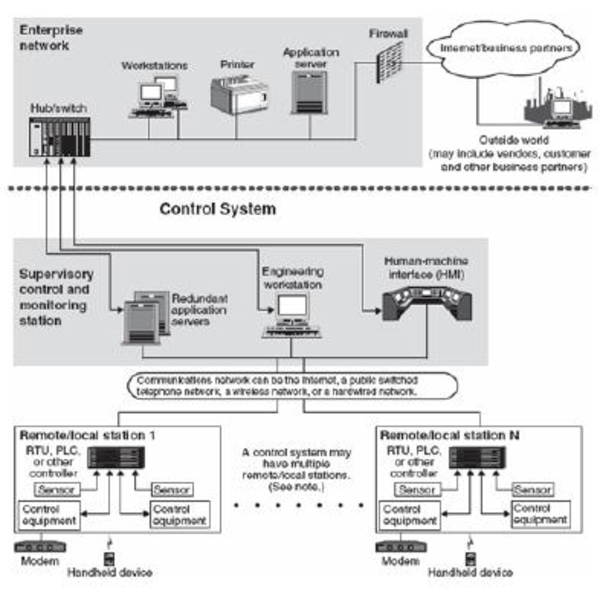
\includegraphics{thesis_files/figure-latex/unnamed-chunk-4-1} 

}

\caption{SCADA components [Zhu2010]}\label{fig:unnamed-chunk-4}
\end{figure}

\subsection{Traffic characterization}\label{traffic-characterization}

As seen in the comparative analysis done in {[}Barbosa2012-1{]}, it is
shown how the traffic greatly differs between SCADA and traditional
networks. Most traffic is generated by automated processes in SCADA
networks as opposed to human-generated traffic predominant in
traditional networks. The traffic pattern generated in SCADA networks
have been found to be fairly static and repetitive, with its network
topology unchanging, or rarely modified. Also seen {[}Cheung2006{]} are
a limited number of applications and protocols that run on industrial
systems. Markedly seen over MODBUS traffic, the messages exchanged
between PLCs are recurrent giving it a fixed pattern and relatively
stationary process.{[}Goldenberg2013{]}{[}Barbosa2012-2,3{]}

\pagebreak

\section{Networking Overview}\label{networking-overview}

In this section, a few fundamental networking terms are discussed.
First, an outline of the OSI model is described, followed by the TCP/IP
and MODBUS/TCP protocols.

\subsection{OSI}\label{osi}

Known as the Open System Interconnection (OSI) model, it was initially
developed by the International Standards Organization (ISO) to define
and characterizes the communication between computing systems. The OSI
model, as shown in Figure 2
(\href{https://engineering.linkedin.com/endorsements/geographic-trends-skills-using-linkedins-endorsement-feature}{Image
source}) is represented as layers, each one expressed as a protocol.
Each layer serves the layer above it, and the lowest one being closest
to the physical medium carrying the communication. Figure OSI Model
depicts each layer and its role and responsibilities.

\begin{figure}

{\centering 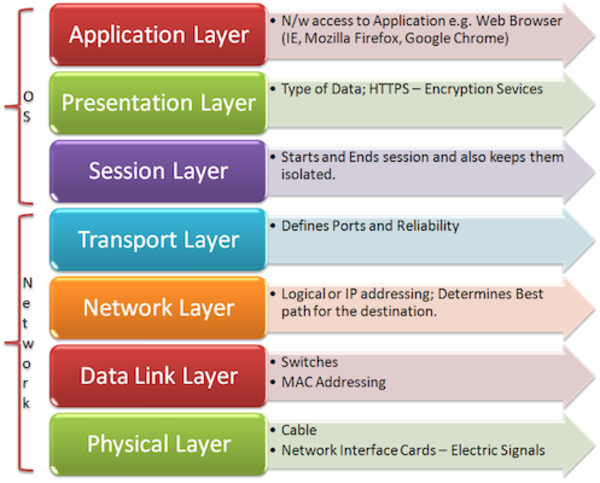
\includegraphics{thesis_files/figure-latex/unnamed-chunk-5-1} 

}

\caption{OSI Model}\label{fig:unnamed-chunk-5}
\end{figure}

\subsection{Protocols}\label{protocols}

As SCADA systems have become increasingly interconnected to enterprise
networks, they operate over, and utilize the same protocols as
previously discussed. Additionally, most SCADA appliances implement and
use the MODBUS/TCP protocol, which run over the TCP protocol.

\subsubsection{Transmission Control Protocol/Internet Protocol
(TCP/IP)}\label{transmission-control-protocolinternet-protocol-tcpip}

Initially developed by the Defense Advanced Research Project Agency
(DARPA) in the late 1960s, the Internet protocol suite was the result of
the research and development of data transmission technologies in the
United States that was used as a standard for military computer
networking.

TCP/IP provides reliable, ordered and error-checked delivery of streams
of octets between applications running on hosts communicating over an IP
network. A detailed illustration of the TCP and IP headers can be seen
in Figures 3
(\href{http://nmap.org/book/images/hdr/MJB-TCP-Header}{Image credit: Max
Baxter}) and Figure 4
(\href{http://nmap.org/book/images/hdr/MJB-IP-Header}{Image credit: Max
Baxter}).

\begin{figure}

{\centering 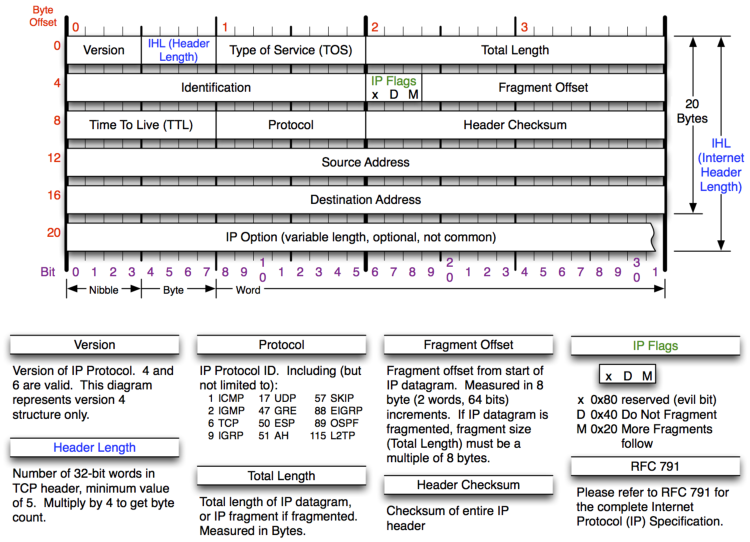
\includegraphics{thesis_files/figure-latex/unnamed-chunk-6-1} 

}

\caption{TCP Header}\label{fig:unnamed-chunk-6}
\end{figure}

\begin{figure}

{\centering 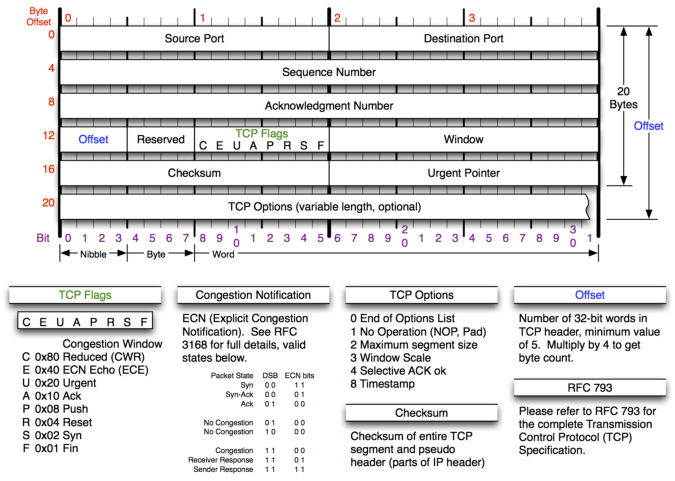
\includegraphics{thesis_files/figure-latex/unnamed-chunk-7-1} 

}

\caption{IPv4 Header}\label{fig:unnamed-chunk-7}
\end{figure}

\subsubsection{MODBUS/TCP}\label{modbustcp}

The MODBUS/TCP protocol is an open standard and popular network protocol
used for ICS devices. It is a messaging protocol located at the
application layer that was designed to communicate with PLCs in
industrial systems. However, due to the limited resources the PLCs have,
it was created to be a simple protocol that provides no security against
unauthorized commands or interception of data.{[}Modbus2012{]} Figure 5
gives an example architecture for MODBUS TCP communication.

\begin{figure}

{\centering 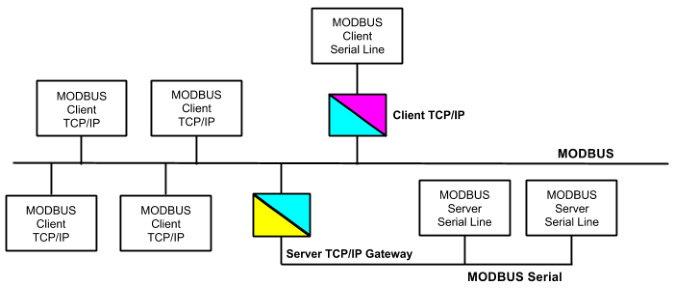
\includegraphics{thesis_files/figure-latex/unnamed-chunk-8-1} 

}

\caption{MODBUS TCP/IP Communication Architecture}\label{fig:unnamed-chunk-8}
\end{figure}

The master initiates a request and the slave sends a response containing
either data or error. The common implementations of MODBUS are over
Ethernet networks (MODBUS/TCP) or Serial busses (MODBUS/RTU). Both forms
of MODBUS contain the packet data unit (PDU), the component consisting
of a function code and data.

Attached to the PDU is the application specific addressing and error
checking, which together comprise the application data unit (ADU).
Specific to MODBUS/TCP, the ADU is encapsulated in the TCP packet.
Thereby eliminating the need to include error checking in the MODBUS/TCP
layer, it is left out from the MODBUS/TCP ADU. The MODBUS/TCP frame is
depicted in Figure 6.

\begin{figure}

{\centering 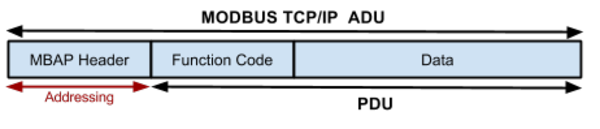
\includegraphics{thesis_files/figure-latex/unnamed-chunk-9-1} 

}

\caption{MODBUS/TCP Frame}\label{fig:unnamed-chunk-9}
\end{figure}

Included in the MODBUS Application Protocol (MBAP) are:

\begin{itemize}
\itemsep1pt\parskip0pt\parsep0pt
\item
  Transaction ID - 2 bytes - identifies request/response pairs
\item
  Protocol ID - 2 bytes - is always 00 00 for Modbus protocol
\item
  Length - 2 bytes - identifies the number of bytes in the following
  message
\item
  Unit ID - 1 byte - used to distinguish which slave is addressed when
  several slaves use the same IP address
\end{itemize}

The MODBUS/TCP transaction ID is reset to zero with each new TCP
session. It is important to note that in identifying MODBUS
conversations, port 502 is reserved for MODBUS communication. MODBUS
requests are initiated from port 502 and MODBUS responses terminate at
port 502.

As a result of using the simple design of MODBUS and its reliance on the
TCP layer, security issues become apparent. With no authentication and
authorization mechanisms, data integrity checks, or encryption, the
SCADA network components provide no identity or permission verification,
message content legitimacy, or confidentiality.

\pagebreak

\section{Common Attacks on SCADA}\label{common-attacks-on-scada}

{[}Hadziosmanovic2010{]}{[}Krotofil2013{]}{[}Lemay2013{]}{[}Rodrigues2011{]}{[}Stouffer2006{]}
define threats and vulnerabilities, security issues, as well as policies
and best practices, and recommendations on how to best secure SCADA
systems. However, cyber attacks continue to increase as SCADA systems
become more exposed and as the attacks grow in sophistication. And
specifically in regards to attacks on MODBUS TCP, little has been
published, except for the work done by Digital Bond\footnote{\url{http://www.digitalbond.com}}.

Leveraging existing enterprise network infrastructure, SCADA systems are
also at risk to the same threats that typical IT systems encounter. In
addition, as SCADA systems are upgraded less frequently and continue to
run on legacy systems, they are rendered even more vulnerable to various
attacks that may be prevented by deploying upgrades that address newer
and known threats. In {[}Zhu2011{]}, outlines and describes in detail
the various methods of cyber attacks on software and hardware and ways
of compromising SCADA systems.

The following provides an overview of common attacks that have been
exploited against SCADA systems {[}Morris2013{]}.

\subsection{Command Injection}\label{command-injection}

In regards to command injection attacks, the attacker may intercept and
alter, or insert conceivably malicious commands that are then
unknowingly executed in the system. Some known types of command
injection attacks are SQL Injection and Cross-Site Scripting (XSS).
False commands meant to alter the control and configuration in ICSs
commonly seen are injected to modify and interrupt communication and
processes.

More frequently seen in SCADA systems, MODBUS communication is
intercepted, or more precisely, an attacker injects MODBUS functions
intended to modify the industrial process.Since the MODBUS/TCP protocol
was not designed with security taken into account and has no encryption
or sophisticated security precautions, it is vulnerable to the
manipulation of the function code or data field sent in the requests.

\subsection{Response Injection}\label{response-injection}

The nature of response injection attacks is that they perform
unauthorized write requests. Commonly used in ICSs, polling is
continuously done in order to audit the state of remote processes. Over
the MODBUS/TCP, there is frequent request and response communication
between the MTU and RTUs. Perpetrators may craft response packets that
are subsequently inserted into the communication loop and if timed
accordingly, is received as the first response to a query thereby
rejecting further responses as invalid.

\subsection{Denial of Service}\label{denial-of-service}

In an attempt to render services unavailable and stop the proper
functioning of a system, denial-of-service attacks either try to bring
down and crash the service, or flood all resources preventing legitimate
users from accessing the service. Attacks of this type on SCADA systems
try to either reboot MODBUS servers or manipulate the controls to take
them out of service. In other cases, an endpoint is overwhelmed to the
point where it cannot take on further requests.

\subsection{Reconnaissance}\label{reconnaissance}

In a reconnaissance attack there is unauthorized reading of data, where
this type of attack generally surveys a network and identifies connected
devices in order to ascertain the network architecture and topology.
Once the network is accessed by the perpetrator, they may carry out
different levels of scanning over the network, such as address, port and
points scanning. In the case of SCADA systems, with the MODBUS/TCP being
the prevailing protocol used for ICS devices, function scanning is also
done.

\subsection{Zero-day Attacks}\label{zero-day-attacks}

Attacks that exploit previously unknown vulnerabilities and security
holes before a vendor can react and correct them via a patch are known
as zero-day attacks. As deploying upgrades and patches to ICSs are
relatively slow and infrequent, ICSs are highly susceptible to the
weakness discovered in software or hardware before they are corrected. A
well-known malware meant to target industrial PLCs, Stuxnet was designed
to exploit an assortment of zero-day flaws.{[}Karnouskos2011{]}

\pagebreak

\section{Intrusion Detection Systems}\label{intrusion-detection-systems}

An intrusion detection system (IDS) is a security mechanism put into
place in order to monitor activity and whose purpose is to identify and
detect any suspicious or unauthorized access or actions to resources and
data. An IDS may act in a passive or reactive manner, the prior in which
unusual activity is logged and an alert is sent to a monitoring system
and the latter where the IDS actively responds to suspicious activity.

Until fairly recently, the application of IDSs to SCADA systems was not
prevalent, however there has been increasing interest and different
approaches and implementations can be seen in the
literature.{[}García2009{]}{[}Yasakethu2013{]}
{[}Wang2011{]}{[}Valdes2009{]}{[}Sayegh2014{]}

The initial model for intrusion detection systems was presented by
{[}Denning1987{]}, where she described the framework for the design and
implementation of a general-purpose intrusion detection system. The
ideal detection system should contain the following characteristics and
have these capabilities {[}Bishop2003{]}:

\begin{itemize}
\itemsep1pt\parskip0pt\parsep0pt
\item
  detect a broad variety of intrusions
\item
  provide detection of intrusions in a timely manner
\item
  analysis should be presented in a simple format
\item
  these tasks must be executed accurately
\end{itemize}

There are two types of IDSs, which are described as follows:

\subsection{Host IDS}\label{host-ids}

Host-based IDSs are placed directly on each individual host to be
monitored and has direct access to the the resources on the host.

\subsection{Network IDS}\label{network-ids}

Network-based IDSs are placed at various strategic points on the network
and the traffic that occur between hosts is inspected by listening to
and analyzing network events.

Threats may be identified by the following means:

\subsubsection{Signature-based}\label{signature-based}

The data captured by the NIDS is examined and compared to an existing
signature database that have attributes of known attacks. Although this
method provides for higher accuracy (less number of false positives) in
detecting known threats, the signature database needs to be continually
maintained and updated frequently.

\subsubsection{Anomaly-based}\label{anomaly-based}

In an anomaly-based NIDS (A-NIDS), any deviation from ``normal''
activity is flagged as an alarm. An initial (normal) profile of the
system is first created where normal activity is observed. Once
established, the A-NIDS collects data from network events and based on
different measures, looks for activity that differs significantly from
the normal profile and raises an alarm. The advantage of an A-NIDS is
that no a priori knowledge is required of previous known attacks and can
be used to define signatures for malicious behaviour, however it cannot
determine a specific attack and has a greater number of false alarms
(false positives) than signature-based IDS.

It is fairly recent to see security devices incorporate anomaly-based
methods, therefore there has been growing research in the methods used
in anomaly detection that try to deal with minimizing the rate of false
positives. The primary methods of anomaly detection are statistical,
data mining, and machine learning, which generally follow through the
stages and are briefly described
below.{[}García2009{]}{[}Yasakethu2013{]}{[}Wang2011{]}

The initial (parameterization) phase of implementing an anomaly-based
detection system is to create the baseline profile of the system
characteristics and behaviour. Then a model is developed using the
training set created using one of the methods outlined below during the
training phase. A comparison of a subset of these methods is given
(Table1).{[}García2009{]} In the final stage, detection of abnormal
behaviour is analyzed by comparing the observed network traffic to the
model. Any significant deviations are signaled and alerted. Figure 7
models this process.

TODO Table1 reference/figure ???

\begin{figure}

{\centering 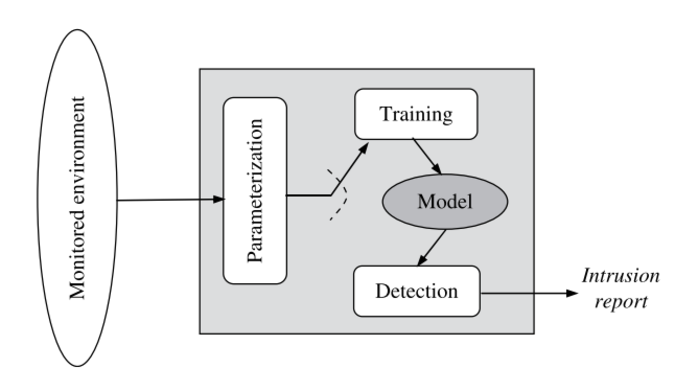
\includegraphics{thesis_files/figure-latex/unnamed-chunk-10-1} 

}

\caption{Functional Architecture of an A-NIDS [García2009]}\label{fig:unnamed-chunk-10}
\end{figure}

\pagebreak

\section{Techniques of Network Intrusion
Detection}\label{techniques-of-network-intrusion-detection}

Numerous anomaly-based methods and techniques have been studied and
implemented in detecting network intrusions. These include statistical,
data mining and machine
learning.{[}García2009{]}{[}Yasakethu2013{]}{[}Wang2011{]}{[}Sousan2011{]}{[}Cheung2007{]}{[}Cunningham2003{]}{[}Fovino2010{]}{[}Kim2013{]}{[}Leandro2014{]}{[}Patcha2007{]}{[}Pathan2014{]}{[}Yang2005{]}{[}Verba2009{]}{[}Verwoerd2002{]}{[}Wang2004{]}{[}Wang2006{]}{[}Mantere2013{]}{[}Yang2014{]}{[}Yu2012{]}{[}Zhou2015{]}
Figure 8 provides a brief summary of these techniques.

\subsection{Statistical}\label{statistical}

Statistical approaches are based on either setting thresholds and
applying them to specific variables, or are based on changes in
distributions over a period of time observed. In the first case, an
upper and lower bound are established to define an appropriate range of
values for the individual variables measured. Earlier methods began by
using the univariate model where single variables are analyzed, and
later, multivariate models were applied, in which highly correlated
metrics were used, as they were considered to be more effective at
distinguishing anomalies. In the second case, considered as a
time-series model, a window of data is used to compute the mean of its
distribution in order to determine the
thresholds.{[}Callegari2008{]}{[}Marchette2003{]}{[}Marchette2004{]}{[}Meza2009{]}
{[}Wang2009{]}{[}Wang2011{]}

\subsection{Data Mining}\label{data-mining}

Data mining, also known as knowledge discovery in databases (KDD), is
the the process of extracting information and detecting interesting
patterns from data. A good deal of work is involved prior to the mining
process in understanding and preparing the data for the mining process
and analysis. Some data mining techniques include, but are not limited
to association rules, language processing, and decision trees and
consist of such algorithms as Apriori, K-Means, and K-Medoids to mention
a few.
{[}Dipali2013{]}{[}Jayasimhan2012{]}{[}Joshi2013{]}{[}Lee1999{]}{[}Lee2001{]}{[}Mara2011{]}
{[}Miao2010{]}{[}Morkhade2013{]}{[}Munz2007{]}{[}Nader2014{]}{[}Niaping2010{]}{[}Singh2013{]}{[}Shukla2014{]}{[}Syarif2012{]}{[}Zhao2010{]}

\subsection{Machine Learning}\label{machine-learning}

In the machine learning approach an algorithm is trained to learn
against a set of data that has been previously identified, or labeled,
and as more data becomes available, the greater the accuracy of the
model. Prominent methods of machine learning are Bayesian and Neural
Networks, SVM, kNN, clustering and outlier
detection.{[}Gao2010{]}{[}Golmah2014{]}{[}Jiang2013{]}{[}Khan2007{]}{[}Linda2009{]}
{[}Maglaras2014{]}{[}Mantere2012{]}{[}Meza2009{]}{[}Mukkamala2006{]}

Similarities and overlap can be seen between the techniques above as
they have evolved and originated from, and are intersections of, the
fields of computer science, statistics, artificial intelligence, and
database systems. Each of these methods presents its advantages and
drawbacks, and in evaluating them, it will be important to consider the
time and complexity in the processing and analysis of data, the
availability of previously identified data, as well as the legibility of
results, that is how easily the results can be read and interpreted.

\begin{figure}

{\centering 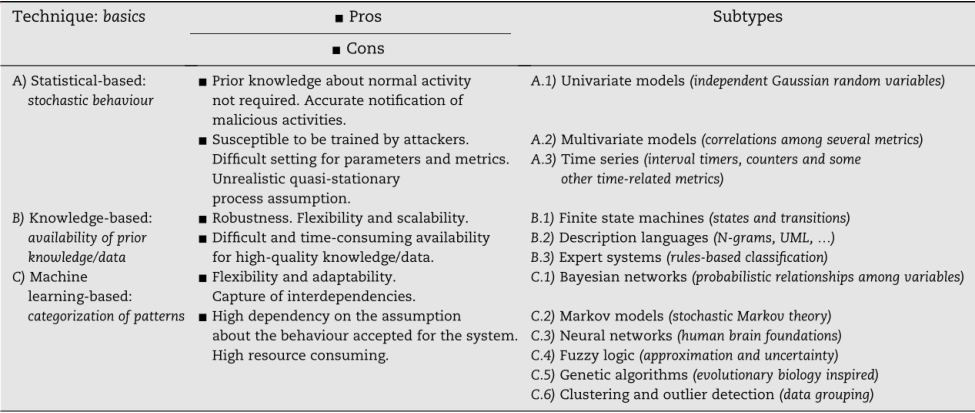
\includegraphics{thesis_files/figure-latex/unnamed-chunk-11-1} 

}

\caption{Fundamentals of the A-NIDS Techniques}\label{fig:unnamed-chunk-11}
\end{figure}

\pagebreak

\section{Tools}\label{tools}

\subsection[Wireshark - Network Traffic Analysis
Tool]{Wireshark\footnote{\url{https://www.wireshark.org/docs/wsug_html_chunked}}
- Network Traffic Analysis
Tool}\label{wireshark2---network-traffic-analysis-tool}

Developed in 1997 by Gerald Combs originally named Ethereal, Wireshark
is now an Open Source GNU project. It is a network packet analyzer, or
``packet sniffer'', that captures and displays network packets.

Captured network packets are saved in the pcap file format and can be
dissected and parsed by Wireshark in order to analyze its contents. An
important aspect of Wireshark is that of its passive/monitoring nature
and so does not send, manipulate, or modify the data passing over the
network.

An initial packet capture file was created over simulated network
traffic using Wireshark. Using its export facilities, various files were
created for further analysis, with information such as TCP endpoints,
conversations, etc.

\subsection[TShark]{TShark\footnote{\url{https://www.wireshark.org/docs/man-pages/tshark.html}}}\label{tshark3}

Another tool from the Wireshark suite is the command-line tool similar
to tcpdump is tshark, a network protocol analyzer. In addition to
capturing packet data over a live network, it is also capable of
analyzing packets from an existing capture file. TShark was used to
parse out various pertinent variables pertaining to the Modbus/TCP
application protocol enclosed in the packet data.

\subsection{UNIX Utilities}\label{unix-utilities}

In order to further parse and transform the data, the UNIX utility tool
sed, which supports the use of regular expressions, was also used.

\subsection[R - Statistical Tool]{R - Statistical Tool\footnote{\url{http://www.r-project.org/}}}\label{r---statistical-tool4}

R is an Open Source programming language and environment used for
statistical computing and graphics. Initially developed by John Chambers
at Bell Labs as the S language in 1993, R was created as a freely
available version under the GNU project by Ross Ihaka and Robert
Gentleman at the University of Auckland, New Zealand.

Maintained by the R Development Core Team and with an active and growing
community, it provides various statistical and graphical creation
capabilities available under most operating systems, and is extensible
with numerous packages available.

\subsection{C/C++}\label{cc}

Originally developed by Dennis Ritchie at AT\&T Bell Labs in the late
60s and early 70s, the C programming language is a low-level, general
purpose computer programming language, that was initially designed for
and implemented on the UNIX OS. A predecessor to the C programming
language is C++, developed by Bjarne Stroustrup in the late 90s. It
inherits most of C's syntax, as well as adds abstraction making it an
object-oriented language.{[}Stroustrup2000{]}

\pagebreak

\section{Data Source}\label{data-source}

It is usual for network data to contain private and sensitive
information, and therefore a limited number of datasets exist for
testing. Consequently, it is difficult to evaluate and assess the
accuracy and validity, as well as to make comparisons across the
different methods applied in anomaly detection.

One of the only publicly available datasets containing network traffic
data has been provided by the US Defense Advanced Research Projects
Agency (DARPA).{[}DARPA1999{]} Network IDS analysis and studies have
commonly been carried out using the DARPA dataset. In this study, the
analysis has been done using data acquired from a simulated testbed, the
Virtual Scada Box.

\subsection{HNS and Virtual Scada Box}\label{hns-and-virtual-scada-box}

Diateam has developed a system, Hynesim (HNS), that is a distributed
platform used in simulating complex information and network systems.
With its ergonomic graphical user interface, Hynesim has a distributed
architecture and modular system, which allows for the inter-connection
between real, as well as virtual systems.

Incorporated into Virtual Scada Box, Hynesim is used to create a virtual
system that simulates a water treatment plant. Virtual Scada Box
includes components such as the PLCs, HMIs, and a virtual water pump
that have been connected over a TCP/IP network.

Data from the simulated network running on the Virtual Scada Box was
used in the analysis. A packet capture file was created via Wireshark,
which captured the network traffic simulated over a virtual SCADA
network. Once the network traffic was captured and saved in a pcap file,
Wireshark provides the capability to export the raw data into various
comma delimited files in order to do further analysis. Exported files
were created with TCP endpoints, TCP conversations, as well as the
entire pcap file, each as a CSV file. (Appendix A)

\subsection[PCAP]{PCAP\footnote{\url{https://www.winpcap.org/ntar/draft/PCAP-DumpFileFormat.html}}}\label{pcap5}

This section describes the format used for the packet capture file
format of the dumped packets. The general structure is in a block format
as shown below.

\pagebreak

\begin{verbatim}

0                   1                   2                   3
0 1 2 3 4 5 6 7 8 9 0 1 2 3 4 5 6 7 8 9 0 1 2 3 4 5 6 7 8 9 0 1
+-+-+-+-+-+-+-+-+-+-+-+-+-+-+-+-+-+-+-+-+-+-+-+-+-+-+-+-+-+-+-+-+
|                          Block Type                           |
+-+-+-+-+-+-+-+-+-+-+-+-+-+-+-+-+-+-+-+-+-+-+-+-+-+-+-+-+-+-+-+-+
|                      Block Total Length                       |
+-+-+-+-+-+-+-+-+-+-+-+-+-+-+-+-+-+-+-+-+-+-+-+-+-+-+-+-+-+-+-+-+
/                          Block Body                           /
/          /* variable length, aligned to 32 bits */            /
+-+-+-+-+-+-+-+-+-+-+-+-+-+-+-+-+-+-+-+-+-+-+-+-+-+-+-+-+-+-+-+-+
|                      Block Total Length                       |
+-+-+-+-+-+-+-+-+-+-+-+-+-+-+-+-+-+-+-+-+-+-+-+-+-+-+-+-+-+-+-+-+    
    
\end{verbatim}

The fields have the following meaning:

\begin{itemize}
\itemsep1pt\parskip0pt\parsep0pt
\item
  Block Type (32 bits) - unique value that identifies the block.
\item
  Block Total Length - total size in bytes.
\item
  Block Body - content.
\item
  Block Total Length - total size in bytes. that is duplicated for
  allowing backward file navigation.
\end{itemize}

\pagebreak

\section{Exploratory Data Analysis}\label{exploratory-data-analysis}

Originally championed by John Tukey{[}Tukey1977{]}, Exploratory Data
Analysis (EDA) is an initial approach to understanding a data set in
order to get a ``feel'' for the data, to summarizing its essential
characteristics and to studying patterns in the data. Moreover,
exploratory data analysis frequently incorporates graphical
representations beyond using quantitative techniques.

Conducting EDA possibly gives further insight into the form and
structure of the data set, in addition to extracting value from it,
visualizing it, and just as importantly, in communicating it. After a
fairly exhaustive study of the state of the art of IDS and SCADA
systems, an initial phase of exploratory data analysis was conducted in
order to better understand the data. This section presents a short list
of statistical terminology, followed by the exploratory data analysis
carried out on the network traffic data captured over the simulated
SCADA network.

\subsection{Statistical Definitions}\label{statistical-definitions}

\subsubsection{Mean}\label{mean}

The (arithmetic) mean is a measure of central tendency, which is a
single value which represents an average of the sample or population. It
is calculated by dividing all the observations by the number of
observations.

\subsubsection{Median}\label{median}

Another measure of central tendency is the median, however, in this
case, the median is determined by first ordering the observations by
magnitude. Then the median is taken as the value which falls in the
middle, or the average of the two middle values in the case of an even
number of observations. The median is better suited when there are
observations, or outliers, that fall way outside the norm. These are
extreme values that differ greatly from other values in the data set.

\subsubsection{Variance}\label{variance}

The variance is the expected value of the squared differences between
the random variables and its mean that is always positive. It gives an
indication of how far apart the values are from the mean and each other.

\[ var[X] = E[(X - E[X])^2] \]

\subsubsection{Standard Deviation}\label{standard-deviation}

The standard deviation is a measure of dispersion, or how spread out a
random variable is around its mean. It is calculated as the square root
of the variance and is, unlike the variance, expressed in the same terms
as the data.

\[ std[X] = \sqrt(var[X]) \]

\subsubsection{Covariance}\label{covariance}

A measure of how closely two variables change, or vary together is the
covariance. Random random variables whose covariance is 0 is said to be
uncorrelated.

\[ cov[X,Y] = E[(X - E[X])(Y-E[Y])] \]

\subsubsection{Correlation}\label{correlation}

Correlation is the strength between the relationship of, or dependence
between, two variables whose value is typically bounded between the
values of -1 and 1, that is to say, that the value has been normalized.
It describes the magnitude and the direction of the relationship. If the
correlation is positive, their values increase together, and if it is
negative, one value decreases as the other value increases.

\[ corr[X,Y] = cov[X,Y] / (std[X]std[Y]) \]

\subsection{Visual Representations}\label{visual-representations}

\subsubsection{Pie chart}\label{pie-chart}

A pie chart is a circular diagram representing numerical proportions as
slices of the pie. Scatter plot A diagram showing a collection of points
as depicted by the coordinates between two variables on a plane. One
axis represents the independent variable, whereas the other represents
the dependent variable.

\subsubsection{Histogram}\label{histogram}

A graphical representation which shows the distribution of continuous
numerical values is a histogram and can be representative of a
probability distribution. A frequency histogram is a univariate
graphical way to show frequency counts of a value depicted with bars of
different heights.

\subsubsection{Bar chart}\label{bar-chart}

Similar to a histogram, a bar chart shows the distribution of values of
a given variable,however, the data is in categorized.

\subsubsection{Boxplot}\label{boxplot}

An effective and graphical method for visualizing outliers is the
boxplot. It displays the data in terms of interquartiles, where outliers
are depicted as individual points. (Figure 9: Boxplot Image
Source{[}Lafaye2013{]})

\begin{figure}

{\centering 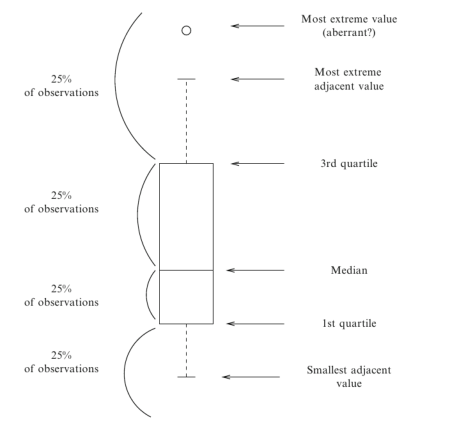
\includegraphics{thesis_files/figure-latex/unnamed-chunk-13-1} 

}

\caption{Boxplot}\label{fig:unnamed-chunk-13}
\end{figure}

\subsubsection{Heat Map}\label{heat-map}

A heat map displays data in a matrix where the values are represented by
a range of colors. Typically displayed in 2D, larger values are usually
shown in darker colors and smaller values in lighter colors on a heat
map. They can also be accompanied by a dendrogram, a tree diagram used
to illustrate clusters.

\subsubsection{Network Graph}\label{network-graph}

Used to model relations between objects, another mathematical structure
is the graph, comprised of nodes, or vertices, and edges. Depending on
the nature of the relationship, a graph may be either cyclic or acyclic,
directed or undirected. Attributes of a node or edge may be reflected in
the graph as well.

\subsection{Data Analysis}\label{data-analysis}

A packet capture file was created via Wireshark, which captured the
network traffic simulated over a virtual SCADA network under normal
conditions (no attacks).

\begin{longtable}[c]{@{}ll@{}}
\toprule\addlinespace
\textbf{capture\_sew\_20150617.pcap} &
\\\addlinespace
\midrule\endhead
\textbf{File} &
\\\addlinespace
Length: & 5124210 bytes
\\\addlinespace
Format: & Wireshark - pcapng
\\\addlinespace
Encapsulation: & Ethernet
\\\addlinespace
Packet size limit: & 65535
\\\addlinespace
\textbf{Time} &
\\\addlinespace
First packet: & 2015-07-21 15:16:56
\\\addlinespace
Last packet: & 2015-07-21 15:29:54
\\\addlinespace
Elapsed: & 00:12:58
\\\addlinespace
\textbf{Traffic Captured} &
\\\addlinespace
Packets & 51358
\\\addlinespace
B/t first and last pkt & 778,118 sec
\\\addlinespace
Avg. packets/sec & 66,003
\\\addlinespace
Avg. packet size & 65,343 bytes
\\\addlinespace
Bytes & 3355887
\\\addlinespace
Avg. bytes/sec & 4312,826
\\\addlinespace
Avg. Mit/sec & 0,035
\\\addlinespace
\bottomrule
\end{longtable}

Once the network traffic was captured and saved in a pcap file,
Wireshark provides the capability to export the raw data into various
comma delimited files in order to do further analysis. Exported files
were created with TCP endpoints, TCP conversations, as well as the
entire pcap file, each as a CSV file. (Appendix A)

\newpage

\subsubsection{Network Analysis}\label{network-analysis}

\paragraph{Protocols}\label{protocols-1}

\begin{figure}

{\centering 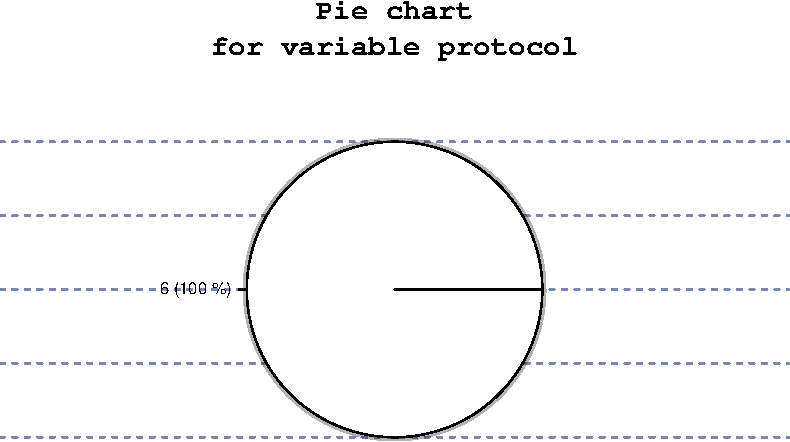
\includegraphics{thesis_files/figure-latex/unnamed-chunk-14-1} 

}

\caption{Pie Chart of Protocols}\label{fig:unnamed-chunk-14}
\end{figure}

\begin{figure}

{\centering 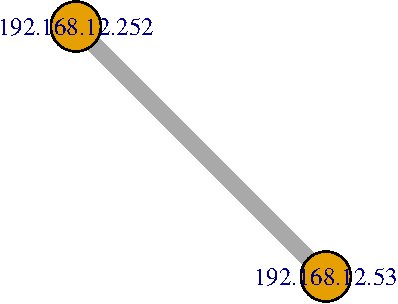
\includegraphics{thesis_files/figure-latex/warning-1} 

}

\caption{SCADA Network Graph}\label{fig:warning}
\end{figure}

\newpage

Source / Destination / UnitID

\begin{verbatim}
           ip.src         ip.dst mbtcp.modbus.unit_id count
1: 192.168.12.117 192.168.12.252                    1 24947
2: 192.168.12.252 192.168.12.117                    1 24945
\end{verbatim}

Sources

\begin{verbatim}
           ip.src count
1: 192.168.12.117 24947
2: 192.168.12.252 24945
\end{verbatim}

Destinations

\begin{verbatim}
           ip.dst count
1: 192.168.12.252 24947
2: 192.168.12.117 24945
\end{verbatim}

Destination / UnitID

\begin{verbatim}
           ip.dst mbtcp.modbus.unit_id   ip.dst.unit_id
1: 192.168.12.252                    1 192.168.12.252/1
2: 192.168.12.117                    1 192.168.12.117/1
\end{verbatim}

Source / Function Code

\begin{verbatim}
           ip.src mbtcp.modbus.func_code         src.func
1: 192.168.12.117                      4 192.168.12.117/4
2: 192.168.12.252                      4 192.168.12.252/4
\end{verbatim}

\newpage

\subsubsection{Packet Analysis}\label{packet-analysis}

\begin{figure}

{\centering 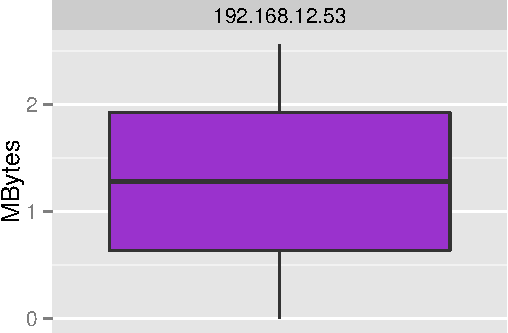
\includegraphics{thesis_files/figure-latex/unnamed-chunk-20-1} 

}

\caption{Source Packet Size Boxplot}\label{fig:unnamed-chunk-20}
\end{figure}

\begin{figure}

{\centering 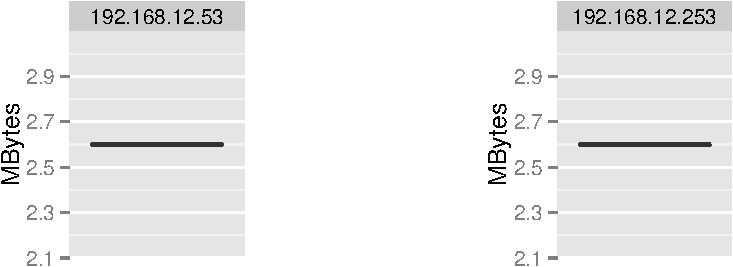
\includegraphics{thesis_files/figure-latex/unnamed-chunk-21-1} 

}

\caption{Bar Charts of Packet Counts}\label{fig:unnamed-chunk-21}
\end{figure}

\paragraph{MODBUS/TCP Request/Response Packet Statistics (Appendix
C)}\label{modbustcp-requestresponse-packet-statistics-appendix-c}

\medskip

MODBUS/TCP \textbf{requests} are identified by packets having
destination port number 502

\begin{figure}

{\centering 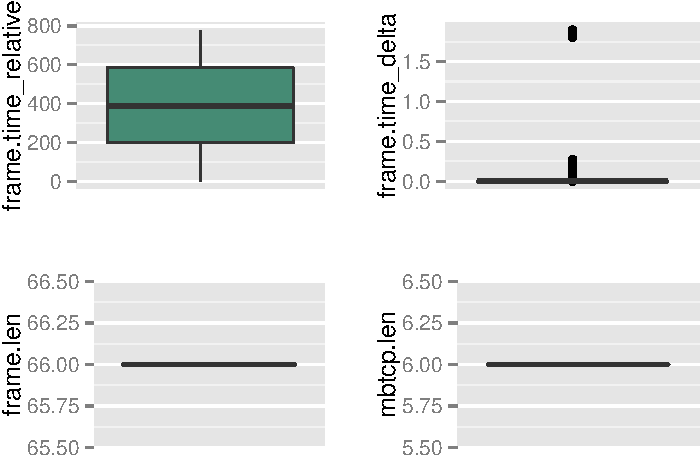
\includegraphics{thesis_files/figure-latex/unnamed-chunk-24-1} 

}

\caption{Boxplot of Request Packets}\label{fig:unnamed-chunk-24}
\end{figure}

MODBUS/TCP \textbf{responses} are identified by packets having source
port number 502

\begin{figure}

{\centering 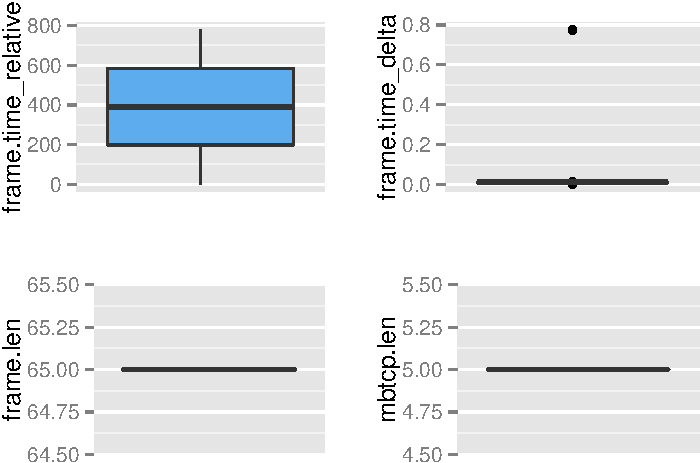
\includegraphics{thesis_files/figure-latex/unnamed-chunk-26-1} 

}

\caption{Boxplot of Response Packets}\label{fig:unnamed-chunk-26}
\end{figure}

\begin{figure}

{\centering 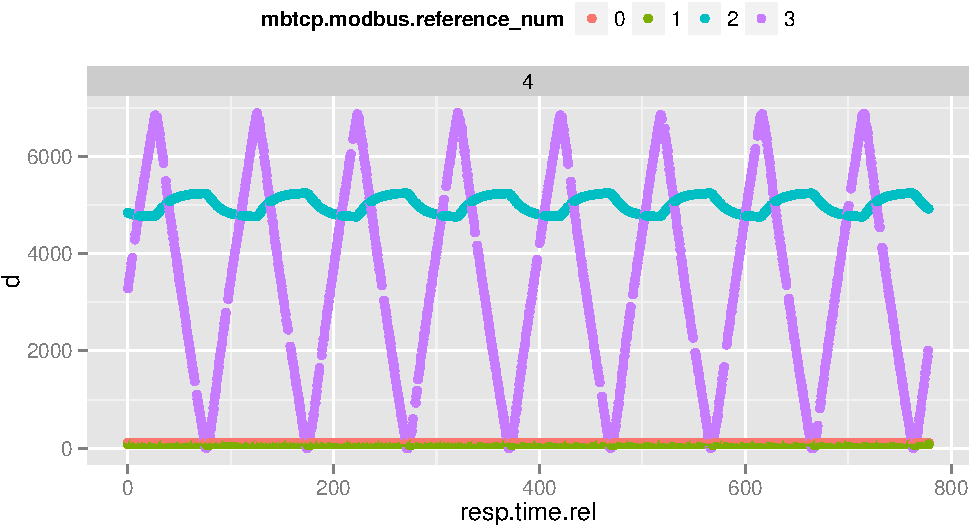
\includegraphics{thesis_files/figure-latex/unnamed-chunk-27-1} 

}

\caption{Scatterplot of Time as a Function of Frame Number}\label{fig:unnamed-chunk-27}
\end{figure}

\begin{figure}

{\centering 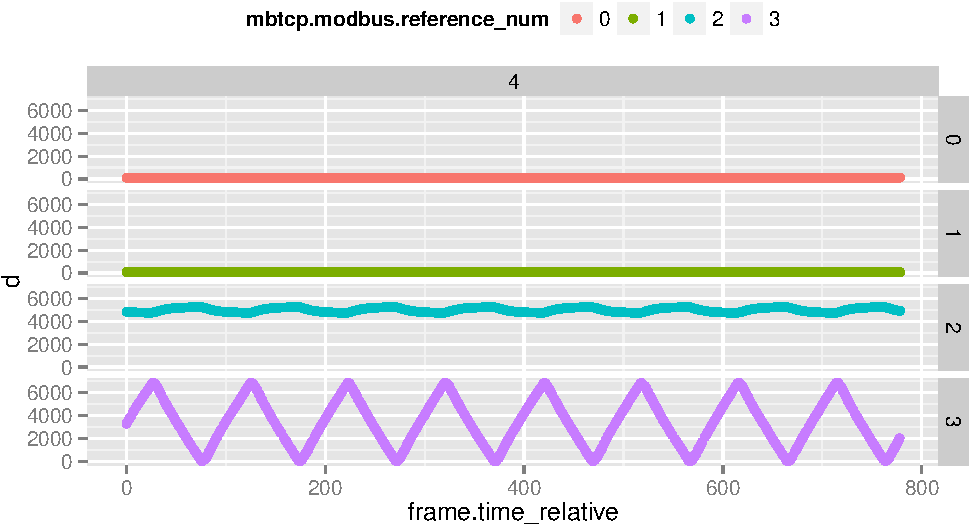
\includegraphics{thesis_files/figure-latex/unnamed-chunk-28-1} 

}

\caption{Boxplot of MODBUS/TCP Data Length}\label{fig:unnamed-chunk-28}
\end{figure}

\subsubsection[MODBUS/TCP Data Analysis]{MODBUS/TCP Data\footnote{\url{https://www.wireshark.org/docs/dfref/m/mbtcp.html}}
Analysis}\label{modbustcp-data6-analysis}

The following analysis was done over the previous dataset that has been
processed to merge response packet to the request packet of the same
transaction. An additional field ``d'' is the data field ``resp.data''
converted from a hex to a decimal value. (Appendix D)

\begin{figure}

{\centering 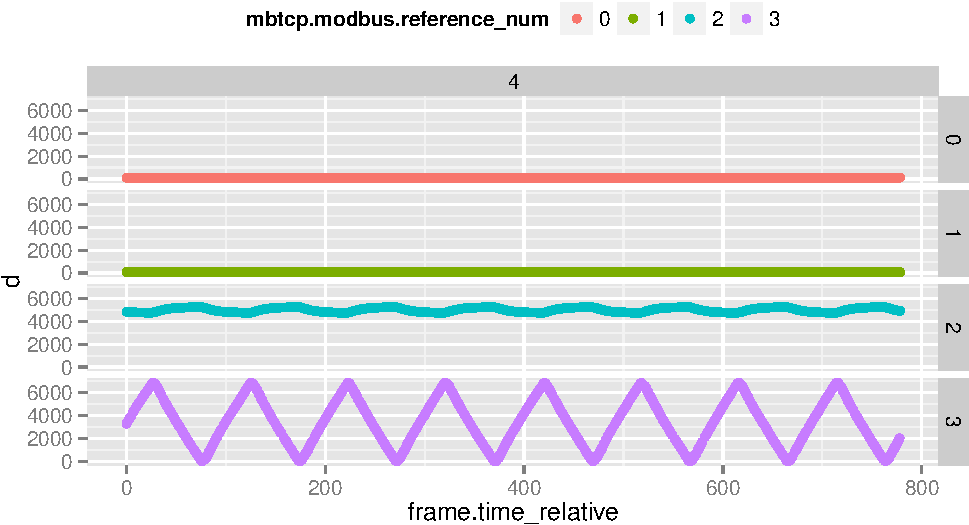
\includegraphics{thesis_files/figure-latex/unnamed-chunk-29-1} 

}

\caption{Graph of MODBUS Data Values over Time by MODBUS  Reference Number}\label{fig:unnamed-chunk-29}
\end{figure}

\begin{figure}

{\centering 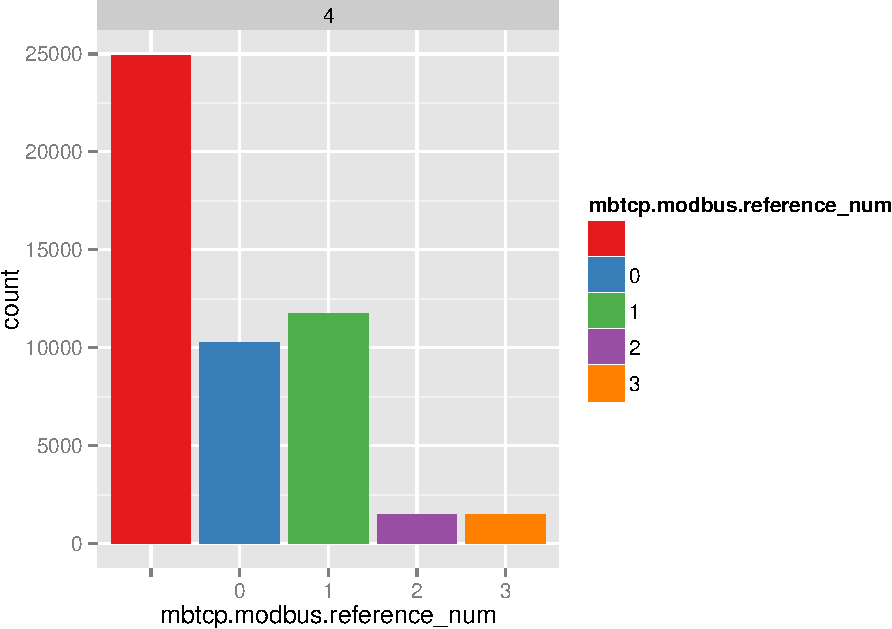
\includegraphics{thesis_files/figure-latex/unnamed-chunk-30-1} 

}

\caption{Graph of MODBUS Data Values over Time by Function Code}\label{fig:unnamed-chunk-30}
\end{figure}

\subsubsection{MODBUS Data Value
Statistics}\label{modbus-data-value-statistics}

\begin{verbatim}
   resp.func.code mbtcp.modbus.reference_num count d.min     d.mean d.max
1:              4                          0 10273   112  112.00000   112
2:              4                          1 11737    64   81.31448    84
3:              4                          2  1468  4758 5005.32493  5242
4:              4                          3  1467     0 3392.64554  6890
          d.sd min.resp.time.rel min.resp.time.rel
1:    0.000000          0.196988          778.1052
2:    3.891773          0.246152          778.1175
3:  179.359760          0.185127          778.0571
4: 2074.517793          0.270168          777.6427
\end{verbatim}

\begin{figure}

{\centering 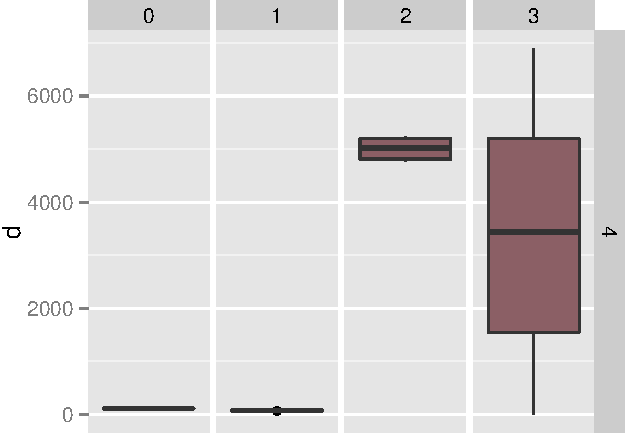
\includegraphics{thesis_files/figure-latex/unnamed-chunk-32-1} 

}

\caption{Bar Chart of MODBUS Reference Numbers by Function Code}\label{fig:unnamed-chunk-32}
\end{figure}

\begin{figure}

{\centering 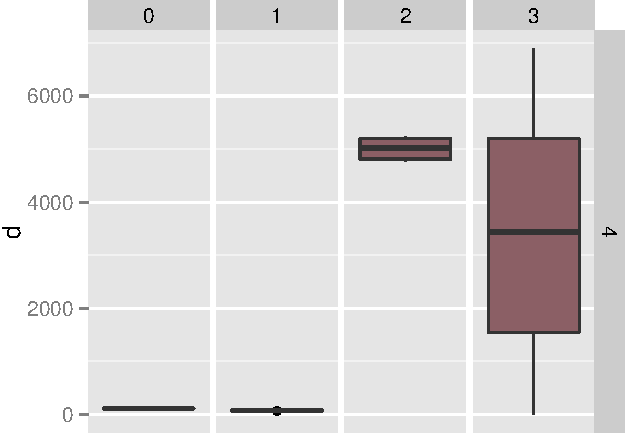
\includegraphics{thesis_files/figure-latex/unnamed-chunk-33-1} 

}

\caption{Boxplot of MODBUS Data Values by Function and Reference Number}\label{fig:unnamed-chunk-33}
\end{figure}

\begin{figure}

{\centering 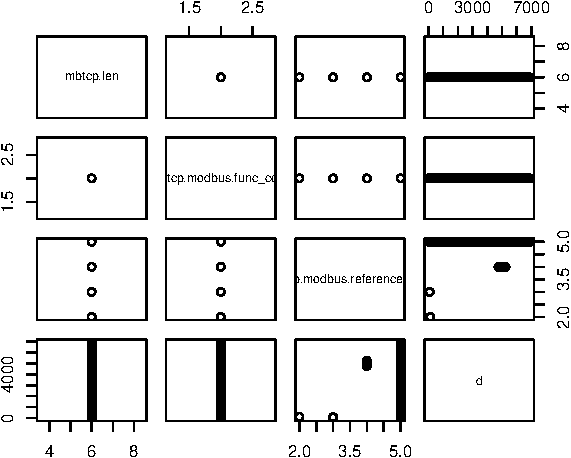
\includegraphics{thesis_files/figure-latex/unnamed-chunk-34-1} 

}

\caption{Scatterplot Matrix of Pairs of Variables}\label{fig:unnamed-chunk-34}
\end{figure}

\begin{figure}

{\centering 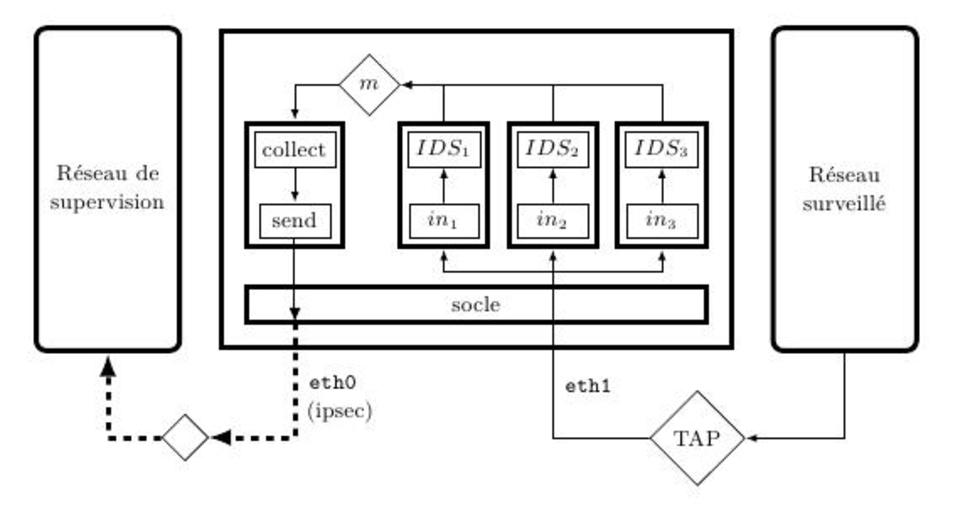
\includegraphics{thesis_files/figure-latex/unnamed-chunk-35-1} 

}

\caption{3D Scatterplot of MODBUS Reference Number
 and Data Over Time for Function Code 4}\label{fig:unnamed-chunk-35}
\end{figure}

\pagebreak

\section{Prototype}\label{prototype}

The SCAD@COPS prototype incorporates the methods as outlined in
{[}Chifflier2014{]}{[}Diallo2014{]}, which define the architectural and
signature-based detection system, and the last component being the
anomaly-based detection system. The signature-based IDS component has
been implemented and configured using Suricata. The initial prototype
will contain an anomaly-based IDS using statistical methods.

\subsection{10.1 Architecture Overview}\label{architecture-overview}

Network IDSs are used for security monitoring, but are themselves also
vulnerable and exposed to attacks. {[}Chifflier2014{]} proposes an
architecture for the IDS sensor devices and software to minimize the
possibility of attacks on it. The two approaches presented are:

\begin{itemize}
\itemsep1pt\parskip0pt\parsep0pt
\item
  reinforce software security- reduce the area of attack, remove unused
  applications and services, and reduce permissions and privileges of
  important processes
\item
  isolate system components- partition and separation between users and
  processes via virtualization
\end{itemize}

In Figure 24, an example is shown of the placement of the IDS and its
supporting DB, connected to other SCADA components.

\begin{figure}

{\centering 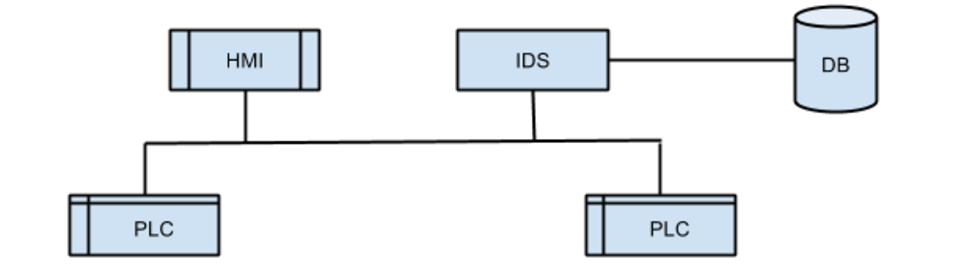
\includegraphics{thesis_files/figure-latex/unnamed-chunk-37-1} 

}

\caption{Technical Architecture}\label{fig:unnamed-chunk-37}
\end{figure}

Based on the recommendations of {[}Chifflier2014{]}, in order to address
the security concerns of the IDS appliance itself, the architecture
contains a partition of the various components and isolates each IDS
instance from one another, as can be seen in Figure 10. All resources
are set to read-only mode, with limited authorized access. For
maintenance, updates are deposited in a dedicated area and then copied
over to another reserved area that are either executed by a scheduled
job or via a trigger. A Mirabox is used as the embedded system running
the latest stable version of Debian and virtual private networks to
communicate between the internal IDS and the supervisory system. (Figure
25)

{[}Diallo2014{]} advises the strategic placement of the monitoring
devices throughout the SCADA system on a dedicated network for
supervision, and presents the two different approaches of a centralized
or a distributed system.

\begin{figure}

{\centering 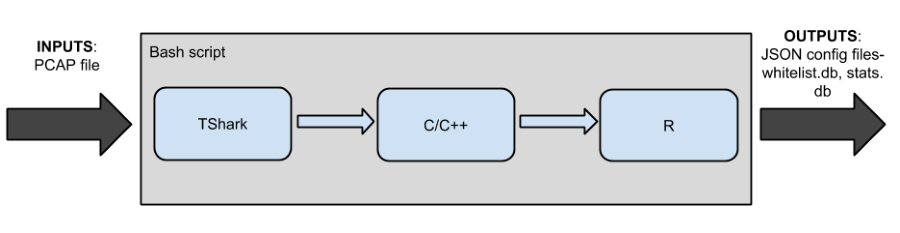
\includegraphics{thesis_files/figure-latex/unnamed-chunk-38-1} 

}

\caption{Architecture of secure IDS [Chifflier2014]}\label{fig:unnamed-chunk-38}
\end{figure}

\subsubsection{Signature-based IDS}\label{signature-based-ids}

In {[}Chifflier2014{]} and {[}Diallo2014{]}, the signature based IDS is
described and the use of the Suricata IDS software with Modbus protocol
are proposed. Rules are configured that conform to, and verify the
correct and normal behaviour of a SCADA system.

\paragraph[Suricata]{Suricata\footnote{\url{http://suricata-ids.org/}}}\label{suricata7}

Essentially the next generation version of Snort, well known and widely
implemented, Suricata is a high performing NIDS, IPS, and network
security monitoring engine. It is based on signatures, however, unlike
Snort has a multithreaded architecture. The advanced techniques embedded
in the engine uses an HTTP normalizer and parser in order to process
HTTP streams which allow it to comprehend traffic at the application
layer of the OSI model.

\subsubsection{Anomaly-based IDS}\label{anomaly-based-ids}

In the scope of the SCAD@COPS project, the anomaly-based component will
be derived from various statistical properties. Section 10.2.2 outlines
the statistical processes, and Section 11 describes the statistical
measures and features.

\subsection{Implementation}\label{implementation}

\subsubsection{Process}\label{process}

Figure 11 shows the steps involved in the entire process from acquiring
the data, computation and analysis, to setting the IDS to detection
mode.

\begin{itemize}
\itemsep1pt\parskip0pt\parsep0pt
\item
  Step 1: Data Acquisition During Normal Activity - From the IDS
  appliance, sniff the network traffic, extract and store data in a
  database.
\item
  Step 2: Statistical Analysis

  \begin{itemize}
  \itemsep1pt\parskip0pt\parsep0pt
  \item
    2.1 - Process data - Perform any transformation, filtering and data
    cleansing necessary.
  \item
    2.2 - Calculate and determine statistical measures.
  \item
    2.3 - Configure appliance with statistical parameters.
  \end{itemize}
\item
  Step 3: Detection Mode - Appliance is set to detection mode.
\end{itemize}

\begin{figure}

{\centering 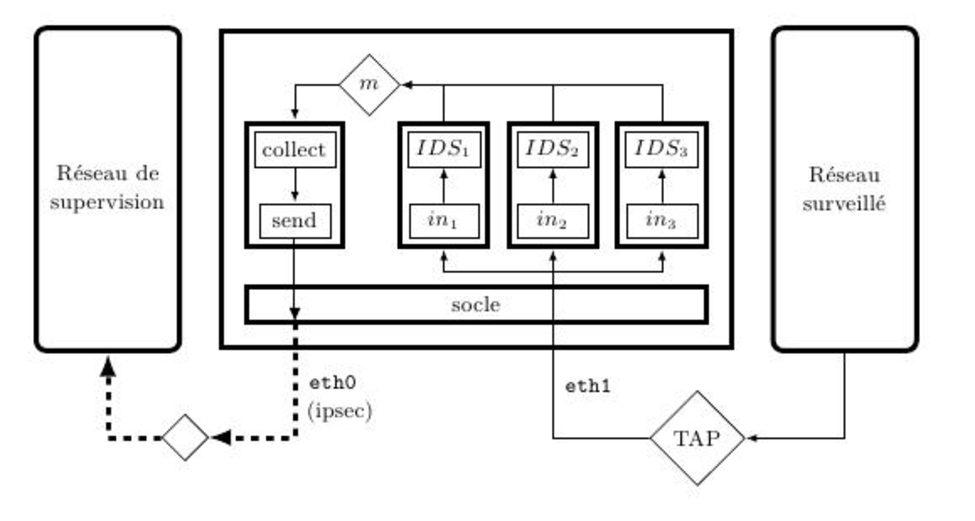
\includegraphics{thesis_files/figure-latex/unnamed-chunk-39-1} 

}

\caption{Process}\label{fig:unnamed-chunk-39}
\end{figure}

\subsubsection{Statistical Processing}\label{statistical-processing}

The statistical process was implemented using various components to
handle specific steps (Figure 26). Each element used was initially
selected to manage a particular task of the process according to its
ease and efficiency of development, as well as its processing time. Once
captured from the monitoring device on the IDS appliance, the packet
capture file is sent to be processed offline. The entire procedure is
handled by a bash script. Most statistical computations were done using
using R scripts, however, part of the data pre-processing, including
merging and transformations went through a C++ program. Configuration
files are subsequently generated in JSON format, which are then uploaded
to the IDS appliance. The components to the process can be found in
Appendix E.

\subsubsection{Modbus/TCP}\label{modbustcp-1}

Example modbus packets:

\paragraph{Query}\label{query}

\begin{verbatim}
65  572.608117000   192.168.12.51   192.168.12.253  Modbus/TCP  66
query: trans:    20; unit:   1, func:   4: Read input registers

0000  00 80 f4 0f 35 aa 00 18  63 37 9b 5b 08 00 45 00   ....5... c7.[..E.
0010  00 34 41 35 40 00 80 06  1f 0e c0 a8 0c 33 c0 a8   .4A5@... .....3..
0020  0c fd 09 c3 01 f6 05 1a  47 65 63 b7 1f c5 50 18   ........ Gec...P.
0030  fa 14 3e 57 00 00 00 14  00 00 00 06 01 04 00 00   ..>W.... ........
0040  00 01    
\end{verbatim}

\paragraph{Response}\label{response}

\begin{verbatim}
66  572.617795000   192.168.12.253  192.168.12.51   Modbus/TCP  65
response: trans:    20; unit:   1, func:   4: Read input registers

0000  00 18 63 37 9b 5b 00 80  f4 0f 35 aa 08 00 45 00   ..c7.[.. ..5...E.
0010  00 33 89 26 40 00 40 06  17 1e c0 a8 0c fd c0 a8   .3.&@.@. ........
0020  0c 33 01 f6 09 c3 63 b7  1f c5 05 1a 47 71 50 18   .3....c. ....GqP.
0030  22 08 9f 5a 00 00 00 14  00 00 00 05 01 04 02 00   "..Z.... ........
0040  75
\end{verbatim}

\pagebreak

\section{Statistical Measures and
Features}\label{statistical-measures-and-features}

Regardless of the predictive method or technique chosen, the predictive
accuracy and performance of any model is influenced by the features
selected, and is therefore important to take into consideration. Feature
selection is the reduction of the input variables. Whether it be in the
field of statistics, data mining, or machine learning, massive amounts
of data that are handled can greatly benefit from the careful selection
of relevant features. In addition, removing redundancies also improves
the efficiency and having both allows for further increased accuracy and
reduction in complexity. However, there should be an appropriate
selection of features so as to prevent any loss of
information.{[}Guyon2003{]}{[}Yu2004{]}

Depending on the size of the dataset and the number of features, or
variables, the selection process may simply be done by a domain expert
who has been trained in a particular field and has the expertise to
determine which features are deemed as important. Although this may be
sufficient in some cases, enormous amounts of data and variables make
the process more complex, and less effective and efficient. More
sophisticated methods go through a learning process in order to detect
patterns with less human intervention.

An example of applying feature selection is in the area of text mining
where unstructured data can be comprised of millions of words. Using
such techniques as stop word elimination and stemming, the
dimensionality is notably reduced.

Network based intrusion detection has been studied for some time and can
be implemented by using conventional network variables.
{[}Ma2008{]}{[}Marchette2004{]} In {[}Mantere2012{]}
{[}Mantere2012{]}{[}Mantere2013{]}, the challenges of feature selection
in the context of anomaly detection in industrial systems are discussed.
The prediction model's performance is highly dependent on the selection
of pertinent variables amongst all available variables, and the feature
set selection detecting any anomalies may be done either manually by one
with knowledge and experience in a domain, or by using other feature
selection techniques not involving humans.

The first version of the SCAD@COPS network intrusion detection device
for industrial systems is based on simple statistical variables that
have been chosen by an expert in the domain of cyber security experience
in SCADA systems. An example configuration file generated from the
statistical process as outlined in Section 10.2.2 (Appendix B) are used
as the parameters in the prototype.

\pagebreak

\section{Testing and Evaluation}\label{testing-and-evaluation}

\begin{itemize}
\itemsep1pt\parskip0pt\parsep0pt
\item
  Test results\\
\item
  Methods of evaluation
\end{itemize}

\pagebreak

\section{Conclusion and Future Work}\label{conclusion-and-future-work}

SCADA systems have typically been isolated and less prone to cyber
threats, but as they continue to increasingly use traditional IT
infrastructure in order to minimize costs and increase efficiency and
functionality, they become more and more vulnerable to cyber attacks.
IDSs offer a solution to provide supervision and protection to SCADA
systems, which are implemented as either host- or network-based IDSs.
Most commercial IDSs offered are usually signature-based, which are only
able to detect previously identified threats and defined rules of
behaviour. A quality of ICSs is that their topology tends to remain
static, their protocols simple, and the traffic fairly regular. The
initial part of this paper provided a general overview of SCADA systems,
networks and protocols, intrusion detection systems

Following, the different techniques of anomaly based network intrusion
detection and tools used in this project were presented. With a growing
need for robust and flexible detection of new threats as the number of
attacks increase, there is more research and advancements in anomaly
detection applying methods such as statistical, data mining and machine
learning techniques to find intelligent ways of anomaly detection. An
integral process also carried out during this work was the exploratory
data analysis phase. This aspect alone can easily, and does typically,
take up a great portion of time as it requires cleaning and treating the
data to be analysed. In addition to the traditional methods of using
descriptive statistics to explain the data, the various graphical and
visual manners of representing the data were presented.

Diateam has proposed a prototype, SCAD@COPS, which is a hybrid IDS that
incorporates both signature-based, as well as an anomaly-based IDS.
Paramount to the mission critical nature of SCADA systems, it is
important for systems to maintain a passive and non-intrusive mode in
detecting intrusions so as not to perturb their functionality. This work
focused its analysis primarily on network data acquired at the TCP/IP
and Ethernet layers. According to research conducted and systems
implemented that can be found in the literature, various techniques have
been examined to detect anomalous behaviour over the network traffic.
These methods and techniques include those of statistical, machine
learning, as well as data mining.

Although the first implementation of the SCAD@COPS NIDS prototype uses
statistical analysis and methods, further research and work can be
conducted to ascertain more viable and effective methods for anomaly
detection. Other areas of study include more sophisticated and advanced
detection of anomalous behaviour applying machine learning techniques
such as Neural and Bayesian networks. Additionally, another potential
area of study is Time-Series analysis. As these methods are fairly new
to the field, more work can be explored and these methods can be
exploited to further improve the accuracy and detection of network
intrusion in future versions of SCAD@COPS.

\pagebreak

\section*{Appendix A}\label{appendix-a}
\addcontentsline{toc}{section}{Appendix A}

\subsection*{Wireshark Exports}\label{wireshark-exports}
\addcontentsline{toc}{subsection}{Wireshark Exports}

Using the export facility in Wireshark, the following are a description
of the exported files:

Entire pcap file exported in CSV format:

\begin{longtable}[c]{@{}l@{}}
\toprule\addlinespace
SCADA\_20150429\_042915.csv
\\\addlinespace
\midrule\endhead
Time
\\\addlinespace
Source
\\\addlinespace
Destination
\\\addlinespace
Protocol
\\\addlinespace
Length
\\\addlinespace
Info
\\\addlinespace
\bottomrule
\end{longtable}

List of endpoints, the traffic to and from an IP address:

\begin{longtable}[c]{@{}l@{}}
\toprule\addlinespace
SCADA\_Security\_042915\_TCP\_Endpoints.csv
\\\addlinespace
\midrule\endhead
Address
\\\addlinespace
Port
\\\addlinespace
Packets
\\\addlinespace
Bytes
\\\addlinespace
Tx.Packets
\\\addlinespace
Tx.Bytes
\\\addlinespace
Rx.Packets
\\\addlinespace
Rx.Bytes
\\\addlinespace
Latitude
\\\addlinespace
Longitude
\\\addlinespace
\bottomrule
\end{longtable}

List of conversations, the traffic between two endpoints :

\begin{longtable}[c]{@{}l@{}}
\toprule\addlinespace
SCADA\_Security\_042915\_TCP\_Conversations.csv
\\\addlinespace
\midrule\endhead
Address.A
\\\addlinespace
Port.A
\\\addlinespace
Address.B
\\\addlinespace
Port.B
\\\addlinespace
Packets
\\\addlinespace
Bytes
\\\addlinespace
Packets.A.B
\\\addlinespace
Bytes.A.B
\\\addlinespace
Packets.A.B.1
\\\addlinespace
Bytes.A.B.1
\\\addlinespace
Rel.Start
\\\addlinespace
Duration
\\\addlinespace
bps.A.B
\\\addlinespace
bps.A.B.1
\\\addlinespace
\bottomrule
\end{longtable}

\pagebreak

\section*{Appendix B}\label{appendix-b}
\addcontentsline{toc}{section}{Appendix B}

\subsection*{Configuration Files}\label{configuration-files}
\addcontentsline{toc}{subsection}{Configuration Files}

Configuration files generated from statistical processing.

\subsection{whitelist.db}\label{whitelist.db}

\begin{verbatim}
{
"IP_SRC" : ["192.168.12.117","192.168.12.252"],
"IP_DST" : ["192.168.12.252","192.168.12.117"],
"IP_MODBUS_UNIT_ID" : [
  "192.168.12.252/1" : {
   "IP_ADDR" : "192.168.12.252",
   "UNIT_ID" : "1 "
  },
  "192.168.12.117/1" : {
   "IP_ADDR" : "192.168.12.117",
   "UNIT_ID" : "1 "
  }
],
"IP_ADDR_MAC_ADDR" : [
  "192.168.12.117/08:00:27:f9:b1:f1" : {
    "IP_ADDR" : "192.168.12.117",
   "MAC_ADDR" : "08:00:27:f9:b1:f1 "
  },
  "192.168.12.252/00:0f:69:0d:55:cd" : {
    "IP_ADDR" : "192.168.12.252",
   "MAC_ADDR" : "00:0f:69:0d:55:cd "
  }
],
"IP_ADDR_MODBUS_FUNC" : [
  "192.168.12.117/4" : {
    "IP_ADDR" : "192.168.12.117",
   "MODBUS_FUNCTION" : "4 "
  },
  "192.168.12.252/4" : {
    "IP_ADDR" : "192.168.12.252",
   "MODBUS_FUNCTION" : "4 "
  }
],
"IP_ADDR_MODBUS_FUNC_REF" : [
  "192.168.12.117/4/0" : {
    "IP_SRC" : "192.168.12.117",
     "MODBUS_FUNCTION" : "4 ",
    "MODBUS_REFERENCE" : "0 "
  },
  "192.168.12.117/4/1" : {
    "IP_SRC" : "192.168.12.117",
     "MODBUS_FUNCTION" : "4 ",
    "MODBUS_REFERENCE" : "1 "
  },
  "192.168.12.117/4/2" : {
    "IP_SRC" : "192.168.12.117",
     "MODBUS_FUNCTION" : "4 ",
    "MODBUS_REFERENCE" : "2 "
  },
  "192.168.12.117/4/3" : {
    "IP_SRC" : "192.168.12.117",
     "MODBUS_FUNCTION" : "4 ",
    "MODBUS_REFERENCE" : "3 "
  }
]
}
\end{verbatim}

\pagebreak

\subsection{stats.db}\label{stats.db}

\begin{verbatim}
{
"SOURCE_DEST_FUNCTION_FREQUENCY" : [
  "192.168.12.117/192.168.12.252/4" : {
    "IP_SRC" : "192.168.12.117",
    "IP_DST" : "192.168.12.252",
    "MODBUS_FUNCTION" : "4 ",
    "FREQUENCY" : "33.170213 "
  }
],
"SOURCE_DEST_FUNCTION_REFERENCE_FREQUENCY" : [
  "192.168.12.117/192.168.12.252/4/0" : {
    "IP_SRC" : "192.168.12.117",
    "IP_DST" : "192.168.12.252",
    "MODBUS_FUNCTION" : "4 ",
    "MODBUS_REFERENCE" : "0 ",
    "FREQUENCY" : "13.715621 "
  },
  "192.168.12.117/192.168.12.252/4/1" : {
    "IP_SRC" : "192.168.12.117",
    "IP_DST" : "192.168.12.252",
    "MODBUS_FUNCTION" : "4 ",
    "MODBUS_REFERENCE" : "1 ",
    "FREQUENCY" : "15.649333 "
  },
  "192.168.12.117/192.168.12.252/4/2" : {
    "IP_SRC" : "192.168.12.117",
    "IP_DST" : "192.168.12.252",
    "MODBUS_FUNCTION" : "4 ",
    "MODBUS_REFERENCE" : "2 ",
    "FREQUENCY" : "1.961230 "
  },
  "192.168.12.117/192.168.12.252/4/3" : {
    "IP_SRC" : "192.168.12.117",
    "IP_DST" : "192.168.12.252",
    "MODBUS_FUNCTION" : "4 ",
    "MODBUS_REFERENCE" : "3 ",
    "FREQUENCY" : "1.971774 "
  }
],
"MODBUS_FUNCTION_REFERENCE_DATA_STATS" : [
  "4/0" : {
    "MODBUS_FUNCTION" : "4",
    "MODBUS_REFERENCE" : "0",
    "D_MIN" : "112.00 ",
    "D_MEAN" : "112.00 ",
    "D_STD_DEV" : "0.00 ",
    "D_MAX" : "112.00 "
  },
  "4/1" : {
    "MODBUS_FUNCTION" : "4",
    "MODBUS_REFERENCE" : "1",
    "D_MIN" : "64.00 ",
    "D_MEAN" : "81.31 ",
    "D_STD_DEV" : "3.89 ",
    "D_MAX" : "84.00 "
  },
  "4/2" : {
    "MODBUS_FUNCTION" : "4",
    "MODBUS_REFERENCE" : "2",
    "D_MIN" : "4758.00 ",
    "D_MEAN" : "5005.44 ",
    "D_STD_DEV" : "179.37 ",
    "D_MAX" : "5242.00 "
  },
  "4/3" : {
    "MODBUS_FUNCTION" : "4",
    "MODBUS_REFERENCE" : "3",
    "D_MIN" : "0.00 ",
    "D_MEAN" : "3392.65 ",
    "D_STD_DEV" : "2074.52 ",
    "D_MAX" : "6890.00 "
  }
]
}
\end{verbatim}

\newpage

\section*{Appendix C}\label{appendix-c}
\addcontentsline{toc}{section}{Appendix C}

\subsection*{MODBUS/TCP Request/Response Packet
Statistics}\label{modbustcp-requestresponse-packet-statistics}
\addcontentsline{toc}{subsection}{MODBUS/TCP Request/Response Packet
Statistics}

\begin{Shaded}
\begin{Highlighting}[]
\KeywordTok{summary}\NormalTok{(requests)}
\end{Highlighting}
\end{Shaded}

\begin{verbatim}
  frame.number   frame.time_relative frame.time_delta     frame.len 
 Min.   :    2   Min.   :  0.1803    Min.   :0.000148   Min.   :66  
 1st Qu.:12838   1st Qu.:198.0391    1st Qu.:0.000277   1st Qu.:66  
 Median :25678   Median :388.5031    Median :0.000350   Median :66  
 Mean   :25678   Mean   :388.8098    Mean   :0.010093   Mean   :66  
 3rd Qu.:38518   3rd Qu.:584.1722    3rd Qu.:0.000376   3rd Qu.:66  
 Max.   :51358   Max.   :778.1178    Max.   :1.893549   Max.   :66  
                                                                    
 ip.proto  ip.version            ip.src                   eth.src     
 6:24947   4:24947    192.168.12.117:24947   00:0f:69:0d:55:cd:    0  
                      192.168.12.252:    0   08:00:27:f9:b1:f1:24947  
                                                                      
                                                                      
                                                                      
                                                                      
                                                                      
            ip.dst                   eth.dst      mbtcp.modbus.unit_id
 192.168.12.117:    0   00:0f:69:0d:55:cd:24947    :    0             
 192.168.12.252:24947   08:00:27:f9:b1:f1:    0   1:24947             
                                                                      
                                                                      
                                                                      
                                                                      
                                                                      
 tcp.srcport  tcp.dstport  mbtcp.prot_id mbtcp.trans_id    mbtcp.len
 1043:24947   1043:    0    :    0       Min.   :  0.0   Min.   :6  
 502 :    0   502 :24947   0:24947       1st Qu.: 64.0   1st Qu.:6  
                                         Median :128.0   Median :6  
                                         Mean   :127.6   Mean   :6  
                                         3rd Qu.:191.0   3rd Qu.:6  
                                         Max.   :255.0   Max.   :6  
                                                                    
 mbtcp.modbus.func_code mbtcp.modbus.reference_num mbtcp.modbus.word_cnt
  :    0                 :    0                    Min.   :1            
 4:24947                0:10273                    1st Qu.:1            
                        1:11739                    Median :1            
                        2: 1468                    Mean   :1            
                        3: 1467                    3rd Qu.:1            
                                                   Max.   :1            
                                                                        
 mbtcp.modbus.data
        :24947    
 00:00  :    0    
 00:07  :    0    
 00:08  :    0    
 00:09  :    0    
 00:0c  :    0    
 (Other):    0    
\end{verbatim}

\begin{Shaded}
\begin{Highlighting}[]
\KeywordTok{summary}\NormalTok{(responses)}
\end{Highlighting}
\end{Shaded}

\begin{verbatim}
  frame.number   frame.time_relative frame.time_delta     frame.len 
 Min.   :    3   Min.   :  0.1851    Min.   :0.001642   Min.   :65  
 1st Qu.:12840   1st Qu.:198.0572    1st Qu.:0.011584   1st Qu.:65  
 Median :25679   Median :388.5154    Median :0.011861   Median :65  
 Mean   :25679   Mean   :388.8184    Mean   :0.011772   Mean   :65  
 3rd Qu.:38518   3rd Qu.:584.1774    3rd Qu.:0.012571   3rd Qu.:65  
 Max.   :51357   Max.   :778.1175    Max.   :0.775146   Max.   :65  
                                                                    
 ip.proto  ip.version            ip.src                   eth.src     
 6:24945   4:24945    192.168.12.117:    0   00:0f:69:0d:55:cd:24945  
                      192.168.12.252:24945   08:00:27:f9:b1:f1:    0  
                                                                      
                                                                      
                                                                      
                                                                      
                                                                      
            ip.dst                   eth.dst      mbtcp.modbus.unit_id
 192.168.12.117:24945   00:0f:69:0d:55:cd:    0    :    0             
 192.168.12.252:    0   08:00:27:f9:b1:f1:24945   1:24945             
                                                                      
                                                                      
                                                                      
                                                                      
                                                                      
 tcp.srcport  tcp.dstport  mbtcp.prot_id mbtcp.trans_id    mbtcp.len
 1043:    0   1043:24945    :    0       Min.   :  0.0   Min.   :5  
 502 :24945   502 :    0   0:24945       1st Qu.: 64.0   1st Qu.:5  
                                         Median :128.0   Median :5  
                                         Mean   :127.6   Mean   :5  
                                         3rd Qu.:191.0   3rd Qu.:5  
                                         Max.   :255.0   Max.   :5  
                                                                    
 mbtcp.modbus.func_code mbtcp.modbus.reference_num mbtcp.modbus.word_cnt
  :    0                 :24945                    Min.   : NA          
 4:24945                0:    0                    1st Qu.: NA          
                        1:    0                    Median : NA          
                        2:    0                    Mean   :NaN          
                        3:    0                    3rd Qu.: NA          
                                                   Max.   : NA          
                                                   NA's   :24945        
 mbtcp.modbus.data
 00:70  :10273    
 00:50  : 5750    
 00:54  : 5561    
 00:40  :  426    
 14:74  :   26    
 12:a0  :   22    
 (Other): 2887    
\end{verbatim}

\newpage

\section*{Appendix D}\label{appendix-d}
\addcontentsline{toc}{section}{Appendix D}

\subsection*{Merged Request/Response Packet
Statistics}\label{merged-requestresponse-packet-statistics}
\addcontentsline{toc}{subsection}{Merged Request/Response Packet
Statistics}

\begin{Shaded}
\begin{Highlighting}[]
\KeywordTok{summary}\NormalTok{(mergedSewDT)}
\end{Highlighting}
\end{Shaded}

\begin{verbatim}
  frame.number   frame.time_relative frame.time_delta     frame.len 
 Min.   :    2   Min.   :  0.1803    Min.   :0.000148   Min.   :66  
 1st Qu.:12839   1st Qu.:198.0456    1st Qu.:0.000277   1st Qu.:66  
 Median :25678   Median :388.5031    Median :0.000350   Median :66  
 Mean   :25678   Mean   :388.8066    Mean   :0.010094   Mean   :66  
 3rd Qu.:38517   3rd Qu.:584.1655    3rd Qu.:0.000376   3rd Qu.:66  
 Max.   :51356   Max.   :778.1055    Max.   :1.893549   Max.   :66  
                                                                    
            ip.src        eth.src                     ip.dst     
               :    0   Length:24945                     :    0  
 192.168.12.117:24945   Class :character   192.168.12.252:24945  
                        Mode  :character                         
                                                                 
                                                                 
                                                                 
                                                                 
   eth.dst          mbtcp.modbus.unit_id tcp.srcport  tcp.dstport
 Length:24945        :    0                  :    0      :    0  
 Class :character   1:24945              1043:24945   502:24945  
 Mode  :character                                                
                                                                 
                                                                 
                                                                 
                                                                 
 mbtcp.prot_id mbtcp.trans_id    mbtcp.len mbtcp.modbus.func_code
  :    0       Min.   :  0.0   Min.   :6    :    0               
 0:24945       1st Qu.: 64.0   1st Qu.:6   4:24945               
               Median :128.0   Median :6                         
               Mean   :127.6   Mean   :6                         
               3rd Qu.:191.0   3rd Qu.:6                         
               Max.   :255.0   Max.   :6                         
                                                                 
 mbtcp.modbus.word_cnt  frame.second   mbtcp.modbus.reference_num
 Min.   :1             Min.   :  0.0    :    0                   
 1st Qu.:1             1st Qu.:198.0   0:10273                   
 Median :1             Median :388.0   1:11737                   
 Mean   :1             Mean   :388.3   2: 1468                   
 3rd Qu.:1             3rd Qu.:584.0   3: 1467                   
 Max.   :1             Max.   :778.0                             
                                                                 
 resp.frame.number resp.time.rel      resp.time.delta       resp.len 
 Min.   :    3     Min.   :  0.1851   Min.   :0.001642   Min.   :65  
 1st Qu.:12840     1st Qu.:198.0572   1st Qu.:0.011584   1st Qu.:65  
 Median :25679     Median :388.5154   Median :0.011861   Median :65  
 Mean   :25679     Mean   :388.8184   Mean   :0.011772   Mean   :65  
 3rd Qu.:38518     3rd Qu.:584.1774   3rd Qu.:0.012571   3rd Qu.:65  
 Max.   :51357     Max.   :778.1175   Max.   :0.775146   Max.   :65  
                                                                     
         resp.ip.src            resp.ip.dst    resp.srcport resp.unit_id
               :    0                 :    0      :    0     :    0     
 192.168.12.252:24945   192.168.12.117:24945   502:24945    1:24945     
                                                                        
                                                                        
                                                                        
                                                                        
                                                                        
 resp.dstport resp.prot_id resp.trans_id   resp.mbcp.len resp.func.code
     :    0    :    0      Min.   :  0.0   Min.   :5      :    0       
 1043:24945   0:24945      1st Qu.: 64.0   1st Qu.:5     4:24945       
                           Median :128.0   Median :5                   
                           Mean   :127.6   Mean   :5                   
                           3rd Qu.:191.0   3rd Qu.:5                   
                           Max.   :255.0   Max.   :5                   
                                                                       
  resp.second      resp.data                resp.eth.src  
 Min.   :  0.0   00:70  :10273   00:0f:69:0d:55:cd:24945  
 1st Qu.:198.0   00:50  : 5750                            
 Median :388.0   00:54  : 5561                            
 Mean   :388.3   00:40  :  426                            
 3rd Qu.:584.0   14:74  :   26                            
 Max.   :778.0   12:a0  :   22                            
                 (Other): 2887                            
            resp.eth.dst         d         
 08:00:27:f9:b1:f1:24945   Min.   :   0.0  
                           1st Qu.:  84.0  
                           Median : 112.0  
                           Mean   : 578.5  
                           3rd Qu.: 112.0  
                           Max.   :6890.0  
                                           
\end{verbatim}

\section*{Appendix E}\label{appendix-e}
\addcontentsline{toc}{section}{Appendix E}

\subsection*{Commands and Scripts}\label{commands-and-scripts}
\addcontentsline{toc}{subsection}{Commands and Scripts}

\subsubsection{TShark}\label{tshark}

Command used to extract various fields from the pcap file used for
analysis.

tshark -r modbus.pcap -T fields -E separator=, -t r -E header=y -e
frame.number -e frame.time\_relative -e frame.time\_delta -e frame.len
-e ip.proto -e ip.version -e ip.src -e eth.src -e ip.dst -e eth.dst -e
mbtcp.modbus.unit\_id -e tcp.srcport -e tcp.dstport -e mbtcp.prot\_id -e
mbtcp.trans\_id -e mbtcp.len -e mbtcp.modbus.func\_code -e
mbtcp.modbus.reference\_num -e mbtcp.modbus.word\_cnt -e
mbtcp.modbus.data \textgreater{} modbus.data

\subsubsection{UNIX}\label{unix}

\paragraph{sed}\label{sed}

Command used to remove empty lines from the pcap data.

sed '/\^{},,,,,.*\$/d' modbus.data \textgreater{} modbus.data

\paragraph{Shell script}\label{shell-script}

processScada.sh - Driver script for statistical computational process.

\paragraph{C/C++ script}\label{cc-script}

processMerge - C/C++ component for handling merge of MODBUS packets in
data processing.

\subsubsection{R}\label{r}

install.R - Setup script to install required packages. sewModbus.R -
Script for processing, analysing and visualizing modbus data.

\newpage

\section*{Bibliography}\label{bibliography}
\addcontentsline{toc}{section}{Bibliography}

{[}Zhu2010{]} B. Zhu and S. Sastry. Scada-specific intrusion
detection/prevention systems: A survey and taxonomy. In Proceedings of
the First Workshop on Secure Control Systems (SCS'10), Stockholm,
Sweden, 2010.

{[}Zhu2011{]} Bonnie Zhu, Anthony Joseph, and Shankar Sastry. 2011. A
Taxonomy of Cyber Attacks on SCADA Systems. In Proceedings of the 2011
International Conference on Internet of Things and 4th International
Conference on Cyber, Physical and Social Computing (ITHINGSCPSCOM '11).
IEEE Computer Society, Washington, DC, USA, 380-388.

{[}Boyer2004{]} S. a. Boyer, ``SCADA - Supervisory And Data
Acquisition.'' The Instrumentation, Systems, and Automation Society,
2004.

{[}Chifflier2014{]} P. Chifflier and A. Fontaine. Architecture système
sécurisée de sonde IDS réseau. C\&ESAR 2014.

{[}Diallo2014{]} David Diallo and M. Feuillet. Détection d'intrusion
dans les systèmes industriels : Suricata et le cas Modbus. C\&ESAR 2014.

{[}Barbosa2012-1{]} R. R. R. Barbosa, R. Sadre, and A. Pras,
``Difficulties in modeling SCADA traffic: A comparative analysis,''
Lect. Notes Comput. Sci. (including Subser. Lect. Notes Artif. Intell.
Lect. Notes Bioinformatics), vol.~7192 LNCS, pp.~126--135, 2012.

{[}Barbosa2012-2{]} R. R. R. Barbosa, R. Sadre, and A. Pras, ``A first
look into SCADA network traffic,'' Proc. 2012 IEEE Netw. Oper. Manag.
Symp. NOMS 2012, pp.~518--521, 2012.

{[}Barbosa2013{]} R. R. R. Barbosa, R. Sadre, and A. Pras, ``Towards
periodicity based anomaly detection in SCADA networks,'' IEEE Int. Conf.
Emerg. Technol. Fact. Autom. ETFA, 2012.

{[}García2009{]} P. García-Teodoro, J. Díaz-Verdejo, G. Maciá-Fernández,
and E. Vázquez. 2009. Anomaly-based network intrusion detection:
Techniques, systems and challenges. Comput. Secur. 28, 1-2 (February
2009), 18-28.

{[}Yasakethu2013{]} Jiang Yasakethu, Intrusion Detection via Machine
Learning for SCADA System Protection. Proceedings of the 1st
International Symposium for ICS \& SCADA Cyber Security Research, 2013.

{[}Wang2011{]} Chengwei Wang; Viswanathan, K.; Choudur, L.; Talwar, V.;
Satterfield, W.; Schwan, K., ``Statistical techniques for online anomaly
detection in data centers,''Integrated Network Management (IM), 2011
IFIP/IEEE International Symposium on , vol., no., pp.385,392, 23-27, May
2011.

{[}Marchette2004{]} D.J. Marchette, Network Intrusion Detection, in
Handbook of Computational Statistics: Concepts and Methods, Gentle,
Hardle and Mori, editors, 2004, 1029-1051, 2004.

{[}Yang2005{]} D. Yang, A. Usynin, and J. Hines, ``Anomaly-based
intrusion detection for SCADA systems,'' 5th Intl. Top. Meet. Nucl.
Plant Instrumentation, Control Hum. Mach. Interface Technol. (NPIC\&HMIT
05), pp.~12--16, 2005.

{[}Callegari2008{]} C. Callegari, S. Vaton, and M. Pagano, ``A new
statistical approach to network anomaly detection,'' pp.~441--447, 2008.

{[}Cheung2007{]} Cheung, S., Dutertre, B., Fong, M., Lindqvist, U.,
Skinner, K., \& Valdes, A. (2007, January). Using model-based intrusion
detection for SCADA networks. InProceedings of the SCADA security
scientific symposium (Vol. 46, pp.~1-12), 2007.

{[}Cunningham2003{]} R. K. Cunningham, S. Cheung, M. Fong, U. Lindqvist,
D. M. Nicol, R. Pawlowski, E. Robinson, W. H. Sanders, S. Singh, A.
Valdes, B. Woodworth, and M. Zhivich, ``Securing Process Control Systems
of Today and Tomorrow *,'' Sci. Technol., no. 2003, pp.~1--24.

{[}Dipali2013{]} Dipali, ``Network Traffic Intrusion Detection System
using Decision Tree \& K-Means Clustering Algorithm,'' vol.~2, no. 5,
pp.~218--220, 2013.

{[}Fovino2010{]} I. N. Fovino, A. Carcano, T. De Lacheze Murel, A.
Trombetta, and M. Masera, ``Modbus/DNP3 state-based intrusion detection
system,'' Proc. - Int. Conf. Adv. Inf. Netw. Appl. AINA, pp.~729--736,
2010.

{[}Gao2010{]} W. Gao, T. Morris, B. Reaves, and D. Richey, ``On SCADA
control system command and response injection and intrusion detection,''
Gen.~Members Meet. eCrime Res. Summit, eCrime 2010, 2010.

{[}Goldenberg2013{]} N. Goldenberg and A. Wool, ``Accurate modeling of
Modbus/TCP for intrusion detection in SCADA systems,'' Int. J. Crit.
Infrastruct. Prot., vol.~6, no. 2, pp.~63--75, 2013.

{[}Golmah2014{]} V. Golmah, ``An Efficient Hybrid Intrusion Detection
System based on C5. 0 and SVM.,'' Int. J. Database Theory Appl., vol.~7,
no. 2, pp.~59--70, 2014.

{[}Hadziosmanovic2010{]} D. Hadˇ, D. Bolzoni, P. H. Hartel, and D.
Hadžiosmanović, ``Towards securing SCADA systems against process-related
threats,'' System, pp.~1--10, 2010.

{[}Jayasimhan2012{]} A. Jayasimhan and J. Gadge, ``Anomaly Detection
using a Clustering Technique,'' Int. J. Appl. Inf. Syst., vol.~2, no. 8,
pp.~5--9, 2012.

{[}Jiang2013{]} J. Jiang, ``Intrusion Detection via Machine Learning for
SCADA System Protection,'' pp.~101--105, 2013.

{[}Joshi2013{]} S. a Joshi and V. S. Pimprale, ``Network Intrusion
Detection System ( NIDS ) based on Data Mining,'' Int. J. Eng. Sci.
Innov. Technol., vol.~2, no. 1, pp.~95--98, 2013.

{[}Karnouskos2011{]} S. Karnouskos, ``Stuxnet worm impact on industrial
cyber-physical system security,'' IECON Proc. (Industrial Electron.
Conf., pp.~4490--4494, 2011.

{[}Khan2007{]} L. Khan, M. Awad, and B. Thuraisingham, ``A new intrusion
detection system using support vector machines and hierarchical
clustering,'' VLDB J., vol.~16, no. 4, pp.~507--521, 2007.

{[}Kim2013{]} S. J. Kim, B. H. Kim, S. S. Yeo, and D. E. Cho, ``Network
anomaly detection for m-connected SCADA networks,'' Proc. - 2013 8th
Int. Conf. Broadband, Wirel. Comput. Commun. Appl. BWCCA 2013,
pp.~351--354, 2013. {[}Krotofil2013{]} M. Krotofil and D. Gollmann,
``Industrial control systems security: What is happening?,'' 2013 11th
IEEE Int. Conf. Ind. Informatics, pp.~664--669, 2013.

{[}Lee1999{]} W. Lee, S. J. Stolfo, and K. W. Mok, ``A Data Mining
Framework for Building Intrusion Detection Models,'' \{IEEE\} Symp.
Secur. Priv., pp.~120--132, 1999.

{[}Lee2001{]} W. L. W. Lee, S. J. Stolfo, P. K. Chan, E. Eskin, W. F. W.
Fan, M. Miller, S. Hershkop, and J. Z. J. Zhang, ``Real time data
mining-based intrusion detection,'' Proc. DARPA Inf. Surviv. Conf. Expo.
II. DISCEX'01, vol.~1, 2001.

{[}Lemay2013{]} A. Lemay, ``Defending the Scada Network Controlling the
Electrical Grid From Advanced Persistent Threats,'' 2013.

{[}Linda2009{]} O. Linda, T. Vollmer, and M. Manic, ``Neural Network
Based Intrusion Detection System for Critical Infrastructures Neural
Networks Neural Network Based Intrusion Detection System for Critical
Infrastructures,'' Neural Networks, 2009.

{[}Leandro2014{]} Leandro A. Maglaras and J. Jiang, ``OCSVM model
combined with K-means recursive clustering for intrusion detection in
SCADA systems,'' vol.~1, pp.~5--6.

{[}Maglaras2014{]} L. A. Maglaras and J. Jiang, ``Intrusion Detection in
SCADA systems using Machine Learning Techniques,'' 2014.

{[}Mantere2012{]} ``Feature Selection for Machine Learning Based Anomaly
Detection in Industrial Control System Networks''. Mantere, 2012

{[}Mantere2012{]} M. Mantere, M. Sailio, and S. Noponen, ``Feature
Selection for Machine Learning Based Anomaly Detection in Industrial
Control System Networks,'' 2012 IEEE Int. Conf. Green Comput. Commun.,
pp.~771--774, 2012.

{[}Mantere2013{]} M. Mantere, M. Sailio, and S. Noponen, ``Network
Traffic Features for Anomaly Detection in Specific Industrial Control
System Network,'' pp.~460--473, 2013.

{[}Mara2011{]} T. Mara, ``The Integration of SNORT with K-Means
Clustering Algorithm to Detect New Attack,'' 2011.

{[}Meza2009{]} J. Meza, S. Campbell, and D. Bailey, ``LBNL Mathematical
and Statistical Opportunities in Cyber Security,'' pp.~1--11, 2009.

{[}Miao2010{]} C. Miao and W. Chen, ``A study of intrusion detection
system based on data mining,'' 2010 IEEE Int. Conf. Inf. Theory Inf.
Secur., pp.~186--189, 2010.

{[}Morkhade2013{]} M. Morkhade and M. Bartere, ``Survey on Data Mining
based Intrusion Detection Systems,'' Ijaiem.Org, vol.~2, no. 3,
pp.~338--343, 2013.

{[}Morris2013{]} T. Morris and W. Gao, ``Industrial Control System Cyber
Attacks,'' \ldots{} Int. Symp. ICS SCADA Cyber \ldots{}, pp.~22--29,
2013.

{[}Munz2007{]} C. Miao and W. Chen, ``A study of intrusion detection
system based on data mining,'' 2010 IEEE Int. Conf. Inf. Theory Inf.
Secur., pp.~186--189, 2010.

{[}Nader2014{]} P. Nader, P. Honeine, and P. Beauseroy, ``-norms in
One-Class Classification for Intrusion Detection in SCADA Systems,''
vol.~10, no. 4, pp.~2308--2317, 2014.

{[}Niaping2010{]} S. N. S. Naiping and Z. G. Z. Genyuan, ``A Study on
Intrusion Detection Based on Data Mining,'' Inf. Sci. Manag. Eng.
(ISME), 2010 Int. Conf., vol.~1, 2010.

{[}Pathan2014{]} A. Pathan, ``The State of the Art in Intrusion
Prevention and Detection,'' Auerbach, 2014.

{[}Yang2014{]} Y. Yang, K. Mclaughlin, S. Sezer, T. Littler, E. G. Im,
B. Pranggono, H. F. Wang, and S. Member, ``Multiattribute SCADA
-Specific intrusion detection system for power networks,'' IEEE Trans.
Power Deliv., vol.~29, no. 3, pp.~1092--1102, 2014.

{[}Yang2014{]} Y. Yang, K. Mclaughlin, S. Sezer, Y. B. Yuan, and W.
Huang, ``Stateful Intrusion Detection for IEC 60870-5-104 SCADA
Security,'' vol.~1, pp.~5--9, 2014.

{[}Yu2012{]} Y. Yu, ``A survey of anomaly intrusion detection
techniques,'' J. Comput. Sci. Coll., pp.~9--17, 2012.

{[}Verba2009{]} J. Verba, ``Idaho national laboratory supervisory
control and data acquisition intrusion detection system (SCADA IDS),''
Int. Conf. Technol. Homel. Secur., no. 208, pp.~469--473, 2008.

{[}Verwoerd2002{]} T. Verwoerd and R. Hunt, ``Intrusion detection
techniques and approaches,'' vol.~25, pp.~1356--1365, 2002.

{[}Wang2006{]} J. Wang and Z. Wang, ``Intrusion Alert Analysis Based on
PCA and the LVQ Neural Network,'' pp.~217--224, 2006.

{[}Wang2004{]} K. Wang and S. Stolfo, ``Anomalous payload-based network
intrusion detection,'' Recent Adv. Intrusion Detect., pp.~203--222,
2004.

{[}Zhao2010{]} D. Z. D. Zhao, Q. X. Q. Xu, and Z. F. Z. Feng, ``Analysis
and Design for Intrusion Detection System Based on Data Mining,'' Educ.
Technol. Comput. Sci. (ETCS), 2010 Second Int. Work., vol.~2, 2010.

{[}Zhou2015{]} C. Zhou, S. Huang, N. Xiong, S. Yang, H. Li, Y. Qin, and
X. Li, ``Design and Analysis of Multimodel-Based Anomaly Intrusion
Detection Systems in Industrial Process Automation,'' pp.~1--16, 2015.

{[}Stouffer2006{]} K. Stouffer, J. Falco, and K. Kent, ``Guide to
supervisory control and data acquisition (SCADA) and industrial control
systems security,'' NIST Spec. Publ. SP800-82, pp.~800--82, 2006.

{[}Rodrigues2011{]} A. Rodrigues, T. Best, and R. Pendse, ``SCADA
security device: design and implementation,'' Proc. Seventh Annu. Work.
Cyber Secur. Inf. Intell. Res., pp.~25:1--25:1, 2011.

{[}Denning1987{]} Denning, D.E., ``An Intrusion-Detection Model,''
Software Engineering, IEEE Transactions on , vol.SE-13, no.2,
pp.222,232, Feb. 1987.

{[}Bishop2003{]} M. Bishop, Computer security: art and science. Boston:
Addison-Wesley, 2003.

{[}Sayegh2014{]} N. Sayegh, I. H. Elhajj, A. Kayssi, and A. Chehab,
``SCADA Intrusion Detection System based on temporal behavior of
frequent patterns,'' MELECON 2014 - 2014 17th IEEE Mediterr.
Electrotech. Conf., no. April, pp.~432--438, 2014.

{[}Valdes2009{]} A. Valdes and S. Cheung, ``Communication pattern
anomaly detection in process control systems,'' 2009 IEEE Conf. Technol.
Homel. Secur. HST 2009, pp.~22--29, 2009.

{[}Singh2013{]} S. Singh and M. Bansal, ``A Survey on Intrusion
Detection System in Data Mining 1 1,2,'' vol.~1, no. 2, pp.~2190--2194,
2013.

{[}Syarif2012{]} I. Syarif, A. Prugel-bennett, and G. Wills,
``Unsupervised clustering approach for network anomaly detection,''
Springer, pp.~135-145, 2012.

{[}Sousan2011{]} W. Sousan, R. Gandhi, Q. Zhu, and W. Mahoney, ``Using
anomalous event patterns in control systems for tamper detection,''
Proc. Seventh Annu. Work. Cyber Secur. Inf. Intell. Res. - CSIIRW '11,
p.~1, 2011.

{[}Shukla2014{]} D. B. Shukla and G. S. Chandel, ``An Implementation Of
Network Traffic Classification Technique Based On K-Medoids,'' vol.~4,
no. 4, pp.~41--46, 2014.

{[}Marchette2003{]} D. J. Marchette, ``Statistical opportunities in
network security,'' in 35th Symposium on the interface, 2003.

{[}Wang2009{]} Wang, Y., Statistical Techniques for Network Security:
Modern Statistically-Based Intrusion Detection and Protection,
Information Science reference, 2009

{[}Meza2009{]} Juan Meza, Scott Campbell, David Bailey, ``Mathematical
and Statistical Opportunities in Cyber Security,'' arXiv preprint
arXiv:0904.1616, 2009.

{[}Mukkamala2006{]} S. Mukkamala, D. Xu, and A. H. Sung, ``Intrusion
Detection Based on Behavior Mining and Machine Learning Techniques,''
pp.~619--628, 2006.

Patcha2007{]} A. Patcha and J. M. Park, ``An overview of anomaly
detection techniques: Existing solutions and latest technological
trends,'' Comput. Networks, vol.~51, no. 12, pp.~3448--3470, 2007.

{[}Modbus2012{]} Modbus application protocol specification v1. 1b3.
North Grafton, Massachusetts (www. modbus. org/specs. php), 2012.

{[}Troy1990{]} Computing fundamentals UNIX systems, Douglas A. Troy,
Addison-Wesley, 1990.

{[}Stroustrup1997{]} Bjarne Stroustrup, The C++ programming language,
Addison-Wesley (Third ed.)., 1997.

{[}DARPA1999{]} DARPA. DARPA Intrusion Detection Evaluation Data Sets,
1999.

{[}Guyon2003{]} Isabelle Guyon, André Elisseeff, ``An Introduction to
Variable and Feature Selection'', Journal of Machine Learning Research,
March 2003

{[}Yu2004{]} Lei Yu, Huan Liu, ``Efficient Feature Selection via
Analysis of Relevance and Redundancy'', Journal of Machine Learning
Research 5, 2004

{[}Ma2009{]} Wanli Ma, ``A Study on the Feature Selection of Network
Traffic for Intrusion Detection Purpose,'' ISI 2008, June 17-20, Taipei,
2008

{[}Tukey1977{]} J.W. Tukey, (1977). Exploratory Data Analysis.
Addison-Wesley. ISBN 0-201-07616-0

{[}Lafaye2013{]} P. Lafaye de Micheaux et al., (2013). The R Software:
Fundamentals of Programming and Statistical Analysis, Statistics and
Computing. Springer New York. ISBN 978-1-4614-9019-7

{[}Stroustrup2000{]} B. Stroustrup, The C++ programming language. 2000.

\pagebreak

{[}1{]}C. Callegari, S. Vaton, and M. Pagano, ``A new statistical
approach to network anomaly detection,'' pp. 441--447, 2008.

{[}2{]}S. Cheung and K. Skinner, ``Using Model-based Intrusion Detection
for SCADA Networks,'' \emph{Science And Technology}, vol. 329, no. 7461,
pp. 1--12, 2006.

\end{document}
